\documentclass[10pt, a4paper]{article}
\usepackage[paper=a4paper, left=3cm, right=3cm, bottom=1.5cm, top=3.5cm]{geometry}
\usepackage[utf8]{inputenc}
\usepackage{verbatim}
\usepackage{mathtools}
\usepackage{float}
%\usepackage{graphicx}
\usepackage[]{algorithm2e}
\usepackage{amssymb}
\usepackage[conEntregas]{caratula}

\usepackage[square,sort,comma,numbers]{natbib}\usepackage{graphicx}
%agregados por anto los proximos, no agregar subcaption xq los bloquea:
\usepackage{enumitem} 
\usepackage{subfigure}

\setcounter{MaxMatrixCols}{12}

\begin{document}

\titulo{RTP1: Sistemas Lineales}

\fecha{28/11/2014}

\materia{M\'etodos Numericos}
%\grupo{Grupo ?}

\integrante{Dellanzo, Claudia Antonella}{019/13}{anto\_tbdt@hotmail.com}
\integrante{De Rocco, Federico}{403/13}{fede.183@hotmail.com}
\integrante{Tallar, Nicol\'as}{218/13}{nicot.sanlorenzo@hotmail.com}
% Pongan cuantos integrantes quieran

\maketitle
\thispagestyle{empty}
\tableofcontents

\newpage
\setcounter{page}{1}
\section{Introducci\'on}

En el siguiente trabajo se presentan distintas implementaciones para la resoluci\'on de sistemas de ecuaciones lineales, utilizando el algoritmo de eliminaci\'on gaussiana y el que se utiliza para la resoluci\'on de estos sistemas cuyas matrices sean bandas, adem\'as de versiones adaptadas de estos para la forma de representar la matrices banda.

El problema que se nos plantea es el de un parabrisas (de determinado largo y ancho) que esta siendo atacado por sanguijuelas que ocasionan que dentro de un determinado radio tenga una cierta temperatura, queriendo nosotros a partir de esta informaci\'on obtener la temperatura de este. Adem\'as sabemos que este parabrisas contiene un sistema de refrigeraci\'on que ocasiona que la temperatura en los bordes sea de -100\hspace{-1.5mm}$\phantom{a}^{\circ}$C, y que si un punto no esta en el borde ni esta afectado directamente por una sanguijuela cumple que (siendo \textit{T(x,y)} la temperatura en el punto \textit{(x,y)}):

\begin{equation}\label{eq:calor}
\frac{\partial^2T(x,y)}{\partial x^{2}}+\frac{\partial^2 T(x,y)}{\partial y^{2}} = 0.
\end{equation}

Con el objetivo de resolver este problema realizamos una discretizaci\'on del parabrisas, teniendo en cuenta solo los puntos de la forma \textit{(j*h,i*h)} (dado un cierto \textit{h $\in$ $\mathbb{R}_{+}$} pasado como par\'ametro) y mediante el m\'etodo de diferencias finitas determinamos que la temperatura en un cierto punto del parabrisas cumple que (siendo \textit{$t_{i,j}$ = T(j*h,i*h)}):
\begin{equation}
t_{ij} \ =\ \frac{ t_{i-1,j} + t_{i+1,j} + t_{i,j-1} + t_{i,j+1}}{4}.\label{eq:calordd}
\end{equation}

Es por ello que luego de todos estos pasos nos queda un sistema de ecuaciones lineales (que posee todas las ecuaciones de las temperaturas de los puntos discretizados del parabrisas), el cual debemos resolver para obtener una aproximaci\'on de la temperatura de ellos. Uno de los puntos, en el cual es primordial saber la temperatura, es el punto cr\'itico, el punto que se encuentra en el centro del parabrisas, debido a que si su temperatura supera los 235\hspace{-1.5mm}$\phantom{a}^{\circ}$C, se romper\'a el parabrisas.

Durante este trabajo, nosotros planteamos dos diferentes alternativas para resolver este sistema (haciendo luego un an\'alisis para realizar una comparaci\'on entre ambas), variando la estructura para representar la matriz asociada a este as\'i como los algoritmos utilizados. Adem\'as nos centramos en el estudio de c\'omo se comporta este sistema y qu\'e dificultades encontramos al tratar de resolverlo, con cuyo fin realizamos una serie de experimentos, pensando previamente a ellos en hip\'otesis y en ver cu\'al iba a ser el resultado y luego comparando esto con lo obtenido. Por \'ultimo buscamos una forma eficiente de eliminar sanguijuelas (es decir que no elimine sanguijuelas de m\'as), analizando su comportamiento y su eficiencia, tambi\'en mediante el uso de experimentos.

\newpage

\section{Matriz Tradicional}
\subsection{Creaci\'on}
El objetivo de este algoritmo es crear la matriz \textit{A} del sistema $Ax=b$, el cual ser\'a utilizado para hallar las temperaturas de todos los puntos discretizados del parabrisas, conteniendo las ecuaciones lineales con las temperaturas de cada punto    discretizado del parabrisas. Para obtener estos puntos vamos recorriendo las filas del parabrisas de abajo hacia arriba (y cada una de ellas de izquierda a derecha). Por cada longitud \textit{h} (pasada como par\'ametro de esta funci\'on) recorrida en el parabrisas, tomaremos esa posici\'on como uno de nuestros puntos discretizados. De esta forma vamos obteniendo estos puntos de manera ordenada para as\'i luego formar la matriz \textit{A} que contendr\'a informaci\'on sobre cada uno de ellos. 

	Este algoritmo va recorriendo estos puntos discretizados hallados y colocando en la matriz \textit{A} determinados valores para cada uno de ellos (los cuales explicaremos posteriormente), cuyas dimensiones son A $\in$ $\mathbb{R}^{n*m\times n*m}$, siendo $n=\frac{a}{h}+1$ y siendo $m=\frac{b}{h}+1$ (\textit{a} el ancho en metros del parabrisas, \textit{b} el largo en metros y \textit{h} la longitud de cada intervalo de discretizaci\'on), donde las filas de \textit{A} representan los puntos discretizados y las columnas los coeficientes que acompañan a las inc\'ognitas de la ecuaci\'on para obtener la temperatura de cada punto discretizado. 

	De esta forma obtenemos el sistema $Ax=b$, en donde la $fila_{k}(A)$ tiene los coeficientes acompañan a las inc\'ognitas de la ecuaci\'on para obtener la temperatura de cada uno de los puntos del sistema, en el orden en el que los recorremos explicado anteriormente. Luego, si este punto se encuentra en la fila \textit{i} y la columna \textit{j} del parabrisas discretizado, la ecuaci\'on que le corresponde es (si es que no se encuentra en el borde ni posee ninguna sanguijuela arriba):

\begin{center}
	$t_{ij}=\frac{t_{(i)(j-1)}+t_{(i)(j+1)}+t_{(i+1)(j)}+t_{(i-1)(j)}}{4}$
\end{center}

Lo que realizamos como paso siguiente es pasar el 4 multiplicando hacia la izquierda y luego el $4*t_{ij}$ restando a derecha, obteniendo lo siguiente:
\begin{center}
	$0=t_{(i)(j-1)}+t_{(i)(j+1)}+t_{(i+1)(j)}+t_{(i-1)(j)}-4t_{ij}$. 
\end{center}

	De esta forma, ahora podemos describir el $b_{i}$, que es el valor asignado a dicha ecuaci\'on, el cu\'al ser\'a $-100$, \textit{t} \'o 0 dependiendo de si el punto al que discretiza la fila \textit{i} es un punto del parabrisas del borde, tiene sanguijuela englob\'andolo o si no es ninguno de los anteriores, respectivamente. Tambi\'en podemos describir el $x_{k}$ que representa a la inc\'ognita $t_{ij}$ del sistema hallada a trav\'es de la funci\'on \textit{OrdenIncog}. Esta funci\'on, dado un punto \textit{i,j} de la discretizaci\'on y el \textit{n} obtenido anteriormente (cantidad de puntos dicretizados sobre el ancho del parabrisas), nos devuelve un n\'umero que representa la posici\'on en la que se encuentra ese punto buscado a trav\'es de la operaci\'on $(n*i)+j$. Es decir que si buscamos, por ejemplo, el punto $(1,2)$ de la discretizaci\'on (indexando desde 0) y tenemos que hay 5 elementos discretizados por ancho del parabrisas ($n=5$), luego el s\'eptimo elemento del vector \textit{x} representar\'a a la inc\'ognita del punto discretizado buscado $t_{12}$.
	
   Cuando nos encontramos con un punto borde $t_{ij}$, la ecuaci\'on de su temperatura estar\'a dada por $t_{ij}=-100$, luego en el punto de la matriz que representa a dicho punto debemos colocar un 1 puesto que es el coeficiente de dicha ecuaci\'on.  Lo mismo sucede en los puntos en los que hay sanguijuelas, supongamos que en el punto de la fila \textit{i} y columna \textit{j} del parabrisas discretizado se encuentra una de ellas, luego su ecuaci\'on de temperatura ser\'a $t_{ij}=$ \textit{t}, siendo \textit{t} la temperatura que ejerce la sanguijuela sobre el parabrisas, debiendo colocar un 1 en el punto de la matriz que lo representa (obtenido nuevamente con \textit{OrdenIncog}). Siguiendo estos pasos, en todos aquellos puntos que sean bordes o que contengan una sanguijuela afect\'andolos, en nuestra matriz veremos solo un 1 en su fila, luego si en todos los puntos hubiesen sanguijuelas o fuesen puntos bordes, tendr\'iamos una matriz con unos en su diagonal debido a la forma que hemos elegido ordenar las inc\'ognitas, que se encuentra relacionada a c\'omo se fueron tomando los puntos discretizados del parabrisas. Esta es de la siguiente manera: supongamos que tenemos una matriz \textit{M} $\in$ $\mathbb{R}^{2\times 2}$ que representa los puntos discretizados del parabrisas, $M=$
$\bigl(\begin{smallmatrix}
t_{11}&t_{12}\\ t_{21}&t_{22}
\end{smallmatrix} \bigr)$. Entonces, nuestra matriz \textit{A} tendr\'a en la primer fila los coeficientes que acompañan a las inc\'ognitas de la ecuaci\'on de temperatura para el punto discretizado $t_{11}$, la segunda la de $t_{12}$, la tercera la del $t_{21}$ y la cuarta la del $t_{22}$

	Ahora veamos el caso en el que hay un punto no borde o sin sanguijuelas. Por la ecuaci\'on de Laplace vista, la temperatura de estos puntos estar\'a dada por el promedio de las temperaturas de los cuatro puntos que la rodean (por izquierda y derecha, por arriba y abajo). Sabemos que las ecuaciones de las temperaturas de los puntos que lo rodean por izquierda y derecha en nuestra matriz son aquellos que se encuentran por encima y por debajo, por ejemplo supongamos que el punto buscado es el $t_{ij}$, luego el punto que se encuentra a su izquierda lo encontramos en el $ t_{(i)(j-1)}$ y el de su derecha es el $t_{(i)(j+1)}$, y, por como fue creada nuestra matriz, estos puntos se encuentran encima y debajo del punto buscado en la matriz \textit{A}. Ahora basta con encontrar d\'onde se encuentran los otros puntos restantes. El punto que se encuentra encima del buscado est\'a en $t_{(i-1)(j)}$ y el punto que est\'a debajo es el $t_{(i+1)(j)}$. Luego, con nuestra funci\'on OrdenIncog, dado el \textit{i} y el \textit{j} podemos encontrar la posici\'on de estos puntos en la matriz. Como los coeficientes que acompañan a estas inc\'ognitas son 1's, basta con poner 1's en estos cuatro puntos de la matriz puesto que tenemos la ecuaci\'on de la forma:
\begin{center}
	$0=t_{(i)(j-1)}+t_{(i)(j+1)}+t_{(i+1)(j)}+t_{(i-1)(j)}-4t_{ij}$. 
\end{center}
	Para colocar el coeficiente $-4$ que acompaña a la inc\'ognita $t_{ij}$ en la matriz, solo debemos colocarlo en la fila y columna dada por la funci\'on OrdenIncog aplicada a \textit{i} y a \textit{j} (que se encontrar\'a sobre la diagonal). Supongamos que OrdenIncog nos devuelve el valor \textit{l}, luego tendremos en la fila y columna \textit{l} un $-4$ y un 1 en la columna \textit{l}-1, \textit{l}+1, \textit{l}+n y \textit{l}-n de la fila \textit{l}.
	
	De esta forma hemos llegado a tener la matriz completa con todos los coeficientes que acompañan a las inc\'ognitas de las ecuaciones de las temperaturas de cada punto discretizado, con una diagonal completa con 1's y $-4$'s, as\'i no encontraremos ning\'un cero en ella, con el resto completo de 0's salvo por como mucho 4 valores por fila, puesto que el valor de cada ecuaci\'on depende como mucho de 5 inc\'ognitas y, por ende, solo tendremos, como mucho, 5 coeficientes de las inc\'ognitas representados.  Entonces dado los par\'ametros de entrada podemos crearnos una matriz que posee representados todos los puntos discretizados del parabrisas junto con los respectivos coeficientes de cada ecuaci\'on que define su temperatura. 
	
	Luego falta armar el vector de resultados, es decir el \textit{b} de la ecuaci\'on $Ax=b$. Este estar\'a formado como un vector de $\mathbb{R}^{n*m}$, conteniendo en cada fila el resultado correspondiente a la ecuaci\'on que representa. Por ejemplo, dada la ecuaci\'on de temperatura $t_{ij}$, para saber a qu\'e est\'a igualada basta usar la funci\'on OrdenIncog con el \textit{i} y el \textit{j} para hallar en que posici\'on del vector se encuentra dicho valor. Cuando colocamos un punto borde, en el vector resultante deberemos colocar un $-100$ en la posici\'on debida, cuando colocamos un punto con sanguijuelas debemos colocar un \textit{t} y cuando nos encontramos en el caso restante deberemos colocar un $0$. 
	
	A continuaci\'on se presentar\'a un pseudoc\'odigo de lo hablado anteriormente, siendo \textit{A} y \textit{b} la matriz y vector, respectivamente, del sistema $Ax=b$, y $n=\frac{a}{h}+1$ (con \textit{a} el ancho en metros del parabrisas y \textit{h} la longitud del intervalo de cada intervalo de discretizaci\'on):

\begin{algorithm}[H]
\For{Cada fila discretizada del parabrisas}{
  \For{Cada columna  de la fila seleccionada de la discretizaci\'on del parabrisas}{
    \eIf{Es punto borde $\vee$ hay sanguijuela englobando ese punto}{
      //Asumiendo que estamos en la fila \textit{k} de A\;
      Colocar 1 en la columna equivalente a la fila ($A_{kk}=1$) y 0 en las restantes\;
      \eIf{Es punto borde}{
        $b_{k}=-100$\;
      }{
        $b_{k}=t$\;
      }
    }{
    		//Asumiendo que estamos en la fila \textit{k} de A\;
    		Colocar -4 en la columna equivalente a la fila ($A_{kk}=-4$)\;
    		Colocar 1 en las columnas $k+1, k-1, k-n, k+n$ de la fila \textit{k}\;
      	Colocar 0 en el resto de las columnas de la fila \textit{k}\;
      $b_{k}=0$\;
    }
  }
}
\caption{Algoritmo de CrearMatriz}
\end{algorithm} 
	
\subsection{Eliminaci\'on Gaussiana}
 	Es un m\'etodo para poder triangular una matriz, es decir para que, dada una matriz, queden 0's debajo de toda la diagonal (sin incluirla) para que luego su resoluci\'on sea m\'as f\'acil puesto que, como cada columna representa al coeficiente de una inc\'ognita, al tenerla triangulada, para obtener el valor de cada una de ellas solo basta ir despejando desde la \'ultima fila hasta la primera debido a que, a medida que vamos subiendo en la matriz, vamos teniendo cada vez m\'as valores despejados. Para realizar este algoritmo, tuvimos en cuenta que, como trabajamos con aritm\'etica finita, puede suceder que al realizar la resta para poner alg\'un cero a los valores que est\'an debajo de la diagonal, esta no quede con un cero sino que con alg\'un valor muy pequeño. Por esto es que decidimos poner directamente aquellos ceros pues ya sabemos que ese valor pertenece a all\'i. Otro dato a tener en cuenta es c\'omo esta formada la matriz que triangularemos(la cual fue explicada anteriormente). Como su diagonal est\'a formada por 1's y $-4$'s, luego los valores que deberemos poner en 0 son aquellos que se encuentran en las filas que poseen un $-4$ puesto que en las dem\'as ya hay 0's debajo de la diagonal. Ahora consideremos alguna fila de la matriz que sea de aquellas cuyo punto no era borde ni ten\'ia una sanguijuela, es decir aquella en la que encontraremos un $-4$ en su fila, llam\'emosla \textit{i}. Tambi\'en consideremos la fila \textit{$j_{1}$} y \textit{$j_{2}$} que ser\'an aquellas filas menores a \textit{i} (\textit{$j_{1}$} \textless  \textit{i}, \textit{$j_{2}$}  \textless \textit{i} ) por la cual deberemos rest\'arsela a \textit{i} para poner 0's debajo de su diagonal, y supongamos que aquellas filas fueron filas anteriormente trianguladas, es decir que sobre su diagonal (sin incluirla) quedaron dos unos (en este ejemplo supongamos que sucede esto, puede suceder que queden otros n\'umeros all\'i puesto que pudieron haber sido modificados en pasos anteriores de la triangulaci\'on). Como al realizar la resta restaremos la fila \textit{i} por alg\'un m\'ultiplo de la fila \textit{$j_{1}$} y \textit{$j_{2}$}, la \'unica forma de que quede un 0 en la diagonal es que esos m\'ultiplos formen un 4 en combinaci\'on. Luego de estudiar el comportamiento de la matriz, pudimos ver que esto nunca puede suceder pues estas filas \textit{$j_{1}$} y \textit{$j_{2}$} contendr\'an un $-4$ o n\'umeros fraccionarios en sus valores que se encuentren sobre la diagonal de la matriz, cuyas combinaciones nunca ser\'an tales que nos anulen el valor de la diagonal.   Por esta raz\'on, luego de aplicar el algoritmo cl\'asico de Eliminaci\'on Guassiana, nunca quedar\'a un 0 en nuestra diagonal y podremos proceder a realizar la resoluci\'on de manera m\'as sencilla. A continuaci\'on presentaremos el pseudoc\'odigo del algoritmo descripto, siendo \textit{F} una fila de la matriz y \textit{a} la matriz:

\begin{algorithm}[H]
 \For{$i=1 ... n-1$}{
  \For{$j=i+1 ... n$}{
   $m_{i,j}=a_{ji}/a_{ii}$\;
   $F_{j}=F_{j}-(m_{ji}*F_{i})$\;  
  }
 }
\caption{Algoritmo de Eliminaci\'on Gaussiana}
\end{algorithm}

\subsection{Resoluci\'on}
	Una vez triangulada la matriz, la dificultad de resolver el sistema es mucho menor. Sea \textit{A, x} y \textit{b} la matriz y vectores que obtuvimos al crear la matriz (del sistema $Ax=b$), nos crearemos un vector \textit{res} en el cual devolveremos el resultado que buscamos. Deberemos avanzar por la diagonal de la matriz en sentido inverso y despejar la solución, puesto que, al estar triangulada la matriz, en el primer caso tendremos la fila con todos ceros en sus columnas menos en la \'ultima, en el segundo tendremos dos columnas no nulas (de las cuales de una ya sabemos su valor) y as\'i sucesivamente. Sea $b_{n}$ el \'ultimo valor de nuestro vector \textit{b}, sabemos que $A_{nn} \* x_{n}=b_{n}$, entonces $x_{n}=b_{n}/A_{nn}$ y aqu\'i obtuvimos el \'ultimo valor para nuestro vector \textit{res}. Esto parece solo solucionarnos la \'ultima inc\'ognita, pero para poder hacerlo para todos los valores de la diagonal basta con que cada vez que llegues a un resultado, hagamos el remplazo en todos los de mayor fila de los valores ya obtenidos y lo pases restando al vector \textit{b}, es decir que $\forall j \in [i-1$..$0]$, $b_{j}=b_{j}-(A_{ji}*res_{i}$). Luego, al ir avanzando por la diagonal de la matriz en sentido inverso, ya tendremos los valores de las inc\'ognitas que se encuentran a su derecha (a la izquierda solo tendremos ceros) y solo basta poner en la posici\'on correspondiente del vector \textit{res} su valor, el cual ser\'a, suponiendo que estamos en la fila \textit{i}, $\frac{b_{i}}{A_{ii}}$ . En esta parte se podría complicar la resoluci\'on si hubiera ceros en la diagonal por la triangulaci\'on ya que esto nos provocar\'ia que en un caso de las variables no se pueda encontrar un resultado. Pero como fue explicado anteriormente en el apartado de Eliminaci\'on Gaussiana, nunca nos encontraremos en tal caso, por lo que nuestro algoritmo nunca se encontrar\'a con tal dificultad.

A continuaci\'on se presentar\'a un pseudoc\'odigo de lo descripto anteriormente, siendo \textit{A} y \textit{b} la matriz y vector, respectivamente, del sistema $Ax=b$, \textit{res} el vector que contendr\'a el resultado final y \textit{n} la cantidad de filas de la matriz \textit{A}:

\begin{algorithm}[H]
\ \\
\For{$i=n-1$..$0$}{
  $res_{i}=b_{i}/A_{ii}$\ \\
  \For{$j=$i$-1$..$0$}{
    $b_{j}=b_{j}-(A_{ji}*res_{i})$\
  }
}
\caption{Algoritmo de Resolver}
\end{algorithm}
	
\newpage

\section{Matriz Banda}

Al analizar la estructura que tiene la matriz de las ecuaciones lineales obtenida luego de la creaci\'on de esta, utilizando el m\'etodo explicado anteriormente, se puede ver que como la funciones son de la forma:

\begin{center}
\textit{$t_{i,j}$ $=$ t \ \ $t_{i,j}$ $=$ -100 \ o \ $t_{i-1,j}$+$t_{i,j-1}$+$t_{i,j+1}$+$t_{i+1,j}$-4*$t_{i,j}$ $=$ 0  }
\end{center}

Luego, en una misma fila de la matriz de las ecuaciones lineales va a haber como m\'aximo cinco coeficientes distintos de cero (los que acompañan a $t_{i-1,j}$, $t_{i,j-1}$, $t_{i,j}$, $t_{i,j+1}$, $t_{i+1,j}$). Es por ello que luego de realizar los algoritmos y de representar la matriz de la forma que normalmente se usar\'ia nos pusimos a pensar de que manera se podr\'ia representar de forma tal que ahorremos tiempo y espacio.

La primera idea que tuvimos es de representarla utilizando una matriz perteneciente a $\mathbb{R}^{n*m \times 5}$ guardando en cada fila \'unicamente los coeficientes distintos de cero, pero nos dimos cuenta que de esta manera no se pod\'ia realizar la eliminaci\'on gaussiana al tratar de resolver el sistema. Esto se debe a que al realizar las restas entre las filas (durante este algoritmo) hab\'ia coeficientes que no podiamos guardar debido a que no acompañaban a ninguno de las inc\'ognitas mencionadas anteriormente. 

Esto se puede ver en el caso que el parabrisas con el que trabajemos sea de la siguiente forma (siendo los c\'irculos negros sin relleno las posiciones en las que estan ubicadas las sanguijuelas):

\begin{center}
\setlength{\unitlength}{1cm}
\begin{picture}(4,3)
\put(0,0){\textbullet}
\put(1,0){\textbullet}
\put(2,0){\textbullet}
\put(3,0){\textbullet}
\put(0,1){\textbullet}
\put(1,1){\textbullet}
\put(2,1){\textbullet}
\put(3,1){\textbullet}
\put(0,2){\textbullet}
\put(1,2){\textbullet}
\put(2,2){\textbullet}
\put(3,2){\textbullet}
\put(2.1,1.09){\circle{0.7}}
\put(1.1,1.09){\circle{0.7}}
\end{picture}
\end{center}

Para el caso anterior, la matriz obtenida mediante la aplicaci\'on del m\'etodo utilizado para la creaci\'on de la matriz de ecuaciones lineales tradicional (el explicado anteriormente) es la siguiente:

\begin{center}
$\begin{pmatrix}
1 & 0 & 0 & 0 & 0 &  0 &  0 & 0 & 0 & 0 & 0 & 0 \\
0 & 1 & 0 & 0 & 0 &  0 &  0 & 0 & 0 & 0 & 0 & 0 \\
0 & 0 & 1 & 0 & 0 &  0 &  0 & 0 & 0 & 0 & 0 & 0 \\
0 & 0 & 0 & 1 & 0 &  0 &  0 & 0 & 0 & 0 & 0 & 0 \\
0 & 0 & 0 & 0 & 1 &  0 &  0 & 0 & 0 & 0 & 0 & 0 \\
0 & 1 & 0 & 0 & 1 & -4 &  1 & 0 & 0 & 1 & 0 & 0 \\
0 & 0 & 1 & 0 & 0 &  1 & -4 & 1 & 0 & 0 & 1 & 0 \\
0 & 0 & 0 & 0 & 0 &  0 &  0 & 1 & 0 & 0 & 0 & 0 \\
0 & 0 & 0 & 0 & 0 &  0 &  0 & 0 & 1 & 0 & 0 & 0 \\
0 & 0 & 0 & 0 & 0 &  0 &  0 & 0 & 0 & 1 & 0 & 0 \\
0 & 0 & 0 & 0 & 0 &  0 &  0 & 0 & 0 & 0 & 1 & 0 \\
0 & 0 & 0 & 0 & 0 &  0 &  0 & 0 & 0 & 0 & 0 & 1
\end{pmatrix}$
\end{center}

En este caso, si representaramos esta matriz utilizando una perteneciente a $\mathbb{R}^{12\times 5}$ (tal como habiamos hablado previamente) deber\'iamos tener en la fila \textit{i} guardado los valores de las columnas \textit{i-3}, \textit{i-1}, \textit{i}, \textit{i+1} y \textit{i+3} de la matriz anterior (en el caso de que algunos de estos valores sea menor a 1 o mayor a \textit{n*m}, en este caso 12, colocaremos un 0 en esa posici\'on). Al realizar este m\'etodo para la matriz mencionada anteriormente se obtiene la siguiente matriz:

\begin{center}
$\begin{pmatrix}
0 & 0 & 1 & 0 & 0 \\
0 & 0 & 1 & 0 & 0 \\
0 & 0 & 1 & 0 & 0 \\
0 & 0 & 1 & 0 & 0 \\
0 & 0 & 1 & 0 & 0 \\
1 & 1 & -4 & 1 & 1 \\
1 & 1 & -4 & 1 & 1 \\
0 & 0 & 1 & 0 & 0 \\
0 & 0 & 1 & 0 & 0 \\
0 & 0 & 1 & 0 & 0 \\
0 & 0 & 1 & 0 & 0 \\
0 & 0 & 1 & 0 & 0
\end{pmatrix}$
\end{center}

Pero el problema es que al realizar la eliminaci\'on gaussiana de la primera de estas matrices obtenemos una que no puede ser guardada de la forma explicada anteriormente, debido a que en una de las posiciones que nosotros no guardar\'iamos hay valores distintos de cero. Esto se debe a que la matriz obtenida mediante la eliminaci\'on gaussiana es:

\begin{center}
$\begin{pmatrix}
1 & 0 & 0 & 0 & 0 &  0 &  0 & 0 & 0 & 0 & 0 & 0 \\
0 & 1 & 0 & 0 & 0 &  0 &  0 & 0 & 0 & 0 & 0 & 0 \\
0 & 0 & 1 & 0 & 0 &  0 &  0 & 0 & 0 & 0 & 0 & 0 \\
0 & 0 & 0 & 1 & 0 &  0 &  0 & 0 & 0 & 0 & 0 & 0 \\
0 & 0 & 0 & 0 & 1 &  0 &  0 & 0 & 0 & 0 & 0 & 0 \\
0 & 0 & 0 & 0 & 0 & -4 &  1 & 0 & 0 & 1 & 0 & 0 \\
0 & 0 & 0 & 0 & 0 &  0 & -\dfrac{15}{4} & 1 & 0 & \dfrac{1}{4} & 1 & 0 \\
0 & 0 & 0 & 0 & 0 &  0 &  0 & 1 & 0 & 0 & 0 & 0 \\
0 & 0 & 0 & 0 & 0 &  0 &  0 & 0 & 1 & 0 & 0 & 0 \\
0 & 0 & 0 & 0 & 0 &  0 &  0 & 0 & 0 & 1 & 0 & 0 \\
0 & 0 & 0 & 0 & 0 &  0 &  0 & 0 & 0 & 0 & 1 & 0 \\
0 & 0 & 0 & 0 & 0 &  0 &  0 & 0 & 0 & 0 & 0 & 1
\end{pmatrix}$
\end{center}

Esta matriz no puede ser guardada en una perteneciente a $\mathbb{R}^{12\times5}$ de la forma propuesta, debido a que en la fila \textit{7} necesitariamos guardar el valor que esta en la columna \textit{7+2}, el cual no guardar\'iamos con el m\'etodo propuesto. Es por esto que decidimos no utilizar este m\'etodo para ahorrar espacio al guardar las matrices con las que trabajamos y pensar en otro para usar.

Al analizar lo ocurrido con la primera de las ideas, nos dimos cuenta de que era necesario tener representados todos los coeficientes que acompañen a las inc\'ognitas que est\'an entre las que ten\'iamos representadas en la idea anterior. Esto quiere decir que, dado el orden que establecimos entre las inc\'ognitas para la construcci\'on de la matriz tradicional (para el cual construimos la funci\'on \textit{ordenIncog} y del cual hablamos cuando explicamos como realizamos la construcci\'on de la matriz de forma tradicional), estando en la fila \textit{i} representamos los coeficientes que acompañan a las inc\'ognitas que estan en la posici\'on desde \textit{i-n} hasta \textit{i+n} (incluyendo \textit{i-n} y \textit{i+n}), siendo la inc\'ognita \textit{x} un \textit{$t_{i,j}$} tal que \textit{ordenIncog} aplicado a este punto d\'e como resultado \textit{x}. Realizamos esto teniendo en cuenta que si \textit{i $<$ n} o \textit{i+n $>$ m*n} entonces, como va a haber lugares en la fila que no representen a un coeficiente, a estos le ponemos el valor cero. Luego para obtener una fila de la matriz banda lo que hacemos es a partir de la misma fila de la matriz tradicional tomar las \textit{n} columnas antes y despu\'es de la que posee el valor de la diagonal (incluyendo a este \'ultimo). En conclusi\'on la matriz que se obtiene posee \textit{2*n+1} columnas por lo que esta es pertenece a $\mathbb{R}^{n*m\times 2*n+1}$ y posee en la columna \textit{n} los coeficientes que acompañan a la diagonal de la matriz (si es que numeramos la primera columna a partir del cero).

Una propiedad importante por la cual podemos \'unicamente guardar estos valores de la matriz y no tener nunca ning\'un problema al realizar la eliminaci\'on gaussiana, como el que teniamos cuando guardabamos solo 5 valores de cada fila, es que la utilizaci\'on de este m\'etodo mantiene la banda de las matrices. Es decir, que si una matriz solo pose\'ia \textit{n} valores a la izquierda y derecha de la diagonal distintos de cero (con el resto de la matriz llena de ceros), entonces luego de cada paso de eliminaci\'on gaussiana, sigue valiendo esto. Es por esta raz\'on que al realizar la eliminaci\'on gaussiana a una matriz que podiamos guardar de la forma planteada, se sigue podiendo guardar (es decir que todos los coeficientes que no guardamos en la matriz valen cero).

Con el fin de poder implementar esta forma de almacenar y manipular matrices tuvimos que realizar unas modificaciones a los algortimos que permiten pasar del parabrisas, con sanguijuelas en determinados puntos, a la temperatura en cada punto del parabrisas (cambiando lo realizado para cuando manipulamos la matriz de forma tradicional). Estos son los algoritmos de creaci\'on, eliminaci\'on gaussiana y de resolver el sistema para la matriz banda, manteniendo siempre las mismas ideas que se implementaron en los algortimos para la matriz tradicional pero adapt\'andolos para poder usarlos para esta matriz (principalmente realizando un cambio en los \'indices).

\subsection{Creaci\'on}

El objetivo de este algoritmo es que dados los datos de entrada del programa (\textit{a},\textit{b}, la posici\'on de las sanguijuelas entre otros) obtener la matriz banda que guarda todas las ecuaciones lineales del sistema, realizando lo explicado previamente. Para esto, realizamos lo siguiente:

\begin{algorithm}[H]
INPUT: $a \in \mathbb{R}, b \in \mathbb{R}, h \in \mathbb{R}, r \in \mathbb{R}, t \in \mathbb{R}, x \in \mathbb{R}^{k}. y \in \mathbb{R}^{k}$ \\
OUTPUT: $A \in \mathbb{R}^{m*n \times 2*n+1}, b \in \mathbb{R}^{m*n}$ \\
$m=\dfrac{b}{h}+1$\;
$n=\dfrac{a}{h}+1$\;
\For{Cada fila \textit{i} discretizada del parabrisas (empezando de la de m\'as abajo y moviendose para arriba)}{
  \For{Cada columna \textit{j} de la fila seleccionada de la discretizaci\'on del parabrisas (comenzando desde la de m\'as a la izquierda y moviendose para la derecha)}{
    $\alpha=ordenIncog(i,j,n)$\;
    \eIf{En ese punto del parabrisas hay una sanguijuela $\lor$ esta en el borde del parabrisas}{
      $A_{\alpha,n} = 1$\;
      \eIf{Ese punto esta en el borde del parabrisas}{
        $b_{\alpha} = -100$\;
      }{
        $b_{\alpha} = t$\;
      }
    }{
      $A_{\alpha,0} = 1$\;
      $A_{\alpha,n-1} = 1$\;
      $A_{\alpha,n} = -4$\;
      $A_{\alpha,n+1} = 1$\;
      $A_{\alpha,2*n} = 1$\;
      $b_{\alpha} = 0$\;
    }
  }
}
\caption{Algoritmo de crear matrices banda}
\end{algorithm} 

Entonces lo que hacemos es, al igual que para la matriz tradicional, recorrer todos los puntos del parabrisas y ver que ecuaci\'on corresponde para ese punto. Para obtener esta, vemos si es que hay una sanguijuela en este punto o si se trata de un punto en el borde del parabrisas, y de esa forma obtenemos los coeficientes que acompañan a las inc\'ognitas, los cuales ubicamos en la matriz banda de la forma explicada anteriormente. Al ir recorriendo los puntos en el mismo orden que estan ordenadas las inc\'ognitas en nuestra matriz, cuando modificamos la fila correspondiente a ese punto correctamente para cada uno de ellos, queda la matriz banda construida de forma correcta. Para esto aprovechamos que la clase vector viene inicializada en 0 y luego s\'olo modificamos los valores que son distintos de cero (cinco como mucho), viendo la posici\'on que deben ocupar en base al punto que estamos analizando y por como es la estructura de la matriz banda.

Un ejemplo de como funciona este m\'etodo se puede ver si poseemos el siguiente parabrisas (siendo los puntos negros los obtenidos mediante la discretizaci\'on y los c\'irculos sin relleno la posici\'on de las sanguijuelas):

\begin{center}
\setlength{\unitlength}{1cm}
\begin{picture}(3,4)
\put(0,0){\textbullet}
\put(0,1){\textbullet}
\put(0,2){\textbullet}
\put(0,3){\textbullet}
\put(1,0){\textbullet}
\put(1,1){\textbullet}
\put(1,2){\textbullet}
\put(1,3){\textbullet}
\put(2,0){\textbullet}
\put(2,1){\textbullet}
\put(2,2){\textbullet}
\put(2,3){\textbullet}
\put(1.09,2.1){\circle{0.7}}
\put(1.09,1.1){\circle{0.7}}
\end{picture}
\end{center}

En este caso obtendr\'iamos las siguientes matrices:

\begin{table}[h]
\centering
\begin{tabular}{c | c 
}
Matriz Tradicional & Matriz Banda \\
\hline
$\begin{pmatrix}
1 & 0 & 0 & 0 & 0 &  0 &  0 & 0 & 0 & 0 & 0 & 0 \\
0 & 1 & 0 & 0 & 0 &  0 &  0 & 0 & 0 & 0 & 0 & 0 \\
0 & 0 & 1 & 0 & 0 &  0 &  0 & 0 & 0 & 0 & 0 & 0 \\
0 & 0 & 0 & 1 & 0 &  0 &  0 & 0 & 0 & 0 & 0 & 0 \\
0 & 1 & 0 & 1 & -4 & 1 & 0 & 1 & 0 & 0 & 0 & 0\\
0 & 0 & 0 & 0 & 0 & 1 & 0 & 0 & 0 & 0 & 0 & 0 \\
0 & 0 & 0 & 0 & 0 & 0 & 1 & 0 & 0 & 0 & 0 & 0\\
0 & 0 & 0 & 0 & 1 & 0 & 1 & -4 & 1 & 0 & 1 & 0 \\
0 & 0 & 0 & 0 & 0 &  0 &  0 & 0 & 1 & 0 & 0 & 0 \\
0 & 0 & 0 & 0 & 0 &  0 &  0 & 0 & 0 & 1 & 0 & 0 \\
0 & 0 & 0 & 0 & 0 &  0 &  0 & 0 & 0 & 0 & 1 & 0 \\
0 & 0 & 0 & 0 & 0 &  0 &  0 & 0 & 0 & 0 & 0 & 1
\end{pmatrix}$
&
$\begin{pmatrix}
0 & 0 & 0 & 1 & 0 & 0 & 0 \\
0 & 0 & 0 & 1 & 0 & 0 & 0 \\
0 & 0 & 0 & 1 & 0 & 0 & 0 \\
0 & 0 & 0 & 1 & 0 & 0 & 0 \\
1 & 0 & 1 & -4 & 1 & 0 & 1 \\
0 & 0 & 0 & 1 & 0 & 0 & 0 \\
0 & 0 & 0 & 1 & 0 & 0 & 0 \\
1 & 0 & 1 & -4 & 1 & 0 & 1 \\
0 & 0 & 0 & 1 & 0 & 0 & 0 \\
0 & 0 & 0 & 1 & 0 & 0 & 0 \\
0 & 0 & 0 & 1 & 0 & 0 & 0 \\
0 & 0 & 0 & 1 & 0 & 0 & 0
\end{pmatrix}$ \\
\end{tabular}
\end{table}

Como se puede observar en el ejemplo, para poder guardar menos espacio de la matriz lo \'unico que hacemos es \'unicamente guardar la banda de la matriz, lo cual ser\'ia en nuestro caso guardar 3 de los valores a la izquierda de la diagonal y 3 a la derecha para cada fila (en general ser\'ian \textit{n}). De esta forma guardamos \'unicamente los coeficientes necesarios para operar con la matriz sin problemas y ahorrar el m\'aximo espacio posible.


\subsection{Eliminaci\'on Gaussiana}

Luego de ver c\'omo crear la matriz banda, nos pusimos a ver como har\'iamos para solucionar el sistema de ecuaciones lineales representado en la matriz banda. Para esto lo que hacemos es utilizar el algoritmo cl\'asico de eliminaci\'on gaussiana (el mismo que utilizamos para la matriz tradicional) salvo que adaptado a que se trata de una matriz banda, adem\'as de realizar una pequeña modificaci\'on a este. Con este fin, implementamos el siguiente algoritmo:

\begin{algorithm}[H]
INPUT/OUTPUT: $A \in \mathbb{R}^{m*n \times 2*n+1}, b \in \mathbb{R}^{m*n}$ \\
INPUT: $n \in \mathbb{N}, m \in \mathbb{N}$\;
$f = 0$\;
$c = 0$\;
\While{$f<n*m$}{
  \textit{//Buscamos una columna \c en la fila f en la que el coeficiente sea distinto de 0}\;
  \While{$c<n \wedge A_{f,c}==0$}{
      $c=c+1$\;
  }
  \eIf{$c<n$}{
    \textit{//Hacemos que el coeficiente en $A_{f,c}$ sea 0, calculando $Fila_{f} = Fila_{f}-m*Fila_{f-(n-c)}$ (teniendo en cuenta que las filas estan almacenadas de manera distinta a la tradicional)}\;
    $m=\dfrac{A_{f,c}}{A_{f-(n-c),n}}$\;
    $A_{f,c}=0$\;
    \For{$i=(c+1)...(c+n)$}{
      $A_{f,i}=A_{f,i}-(m*A_{f-(n-c),n+(i-c)})$\;
    }
    $b_{f}=b_{f}-(m*b_{f-(n-c)})$\;
    $c=c+1$\;
  }{
    $f=f+1$\;
    $c=0$\;
  }
}
\caption{Eliminaci\'on Gaussiana matriz Banda}
\end{algorithm}

Tal como explicamos antes, el objetivo de este algoritmo es de llevar a cabo la eliminaci\'on gaussiana para matrices representadas mediante la estructura alternativa presentada. Este posee una pequeña diferencia en comparaci\'on con el implementado para las matrices representadas tradicionalmente y con el algoritmo de eliminaci\'on gaussiana, la cual esta explicada en la secci\'on de mejoras.

Como el objetivo de la eliminaci\'on gaussiana es que la matriz pase a ser triangular superior, esto se logra con las matrices banda cuando las primeras \textit{n} columnas quedan con sus valores en cero. Con este fin, en nuestro algoritmo iremos focalizandonos en cada una de las filas, poniendo en cero los valores necesarios antes de pasar a la siguiente. Para hacer esto, en cada paso vamos a poner un nuevo coeficiente de la matriz en cero (de la fila con la que estamos trabajando) si es que hay alguno que debamos poner en cero (es decir alguno localizado en las primeras \textit{n} columnas). Si esto no es cierto, pasamos a la siguiente fila y seguimos con la ejecuci\'on del algoritmo hasta haber recorrido todas las filas. Para poner un cero en la posici\'on \textit{(f,c)} de la matriz banda, lo que hacemos es realizar la siguiente cuenta:

\begin{center}
$m = \dfrac{A_{f,c}}{A_{f-(n-c),n}}$ \\
$Fila_{f} = Fila_{f}-m*Fila_{f-(n-c)}$
\end{center}

Esta se realiza teniendo en cuenta que las filas de las que hablamos son las que representar\'ian las guardadas en la matriz banda, es decir, tomando los valores guardados y agregando los ceros a izquierda y derecha que le corresponder\'ian tener si representaramos a la matriz de forma tradicional. Entonces, al hacer esta cuenta debemos restar el elemento \textit{i} de la fila \textit{f} de \textit{A} con el elemento \textit{n+(i-c)} de la fila \textit{f-(n-c)} (siendo este \'ultimo multiplicado por \textit{m}).

Con esta cuenta nosotros queremos realizar algo similar a lo que se hace en cada uno de los pasos de la eliminaci\'on gaussiana tradicional, es decir dada la posici\'on \textit{(i,j)} en la que nos encontramos en la matriz, encontrar la fila \textit{j} para asi poder restar ambas filas y que quede un cero en esta posici\'on de la matriz (todo esto considerando la matriz que se obtendr\'ia si se buscar\'ia como representar tradicionalmente la matriz banda). Pero como en este caso no queremos realizar este pasaje de como esta representada la matriz (porque sino no aprovechar\'iamos al m\'aximo los beneficios de la utilizaci\'on de las matrices banda), tenemos que buscar alguna forma de ver que fila debemos utilizar. Para esto nos aprovechamos que el n\'umero de filas de esta forma de representar la matriz es el mismo que si utilizaramos el m\'etodo tradicional. Entonces, si quisieramos que quede un cero en la posici\'on \textit{(f,c)} de la matriz banda, si \textit{c} fuera igual a \textit{n} entonces \textit{j} ser\'ia igual a \textit{f} (porque como \textit{c==n} \textit{(i,j)} pertenece a la diagonal de la matriz representada de forma tradicional). Entonces, la diferencia entre \textit{c} y \textit{n} es igual que la diferencia entre \textit{j} y \textit{f} por lo que llegamos a la conclusi\'on que la fila que debemos utilizar con el objetivo de que haya un cero en la posici\'on \textit{(f,c)} es la fila \textit{f-(n-c)}. Entonces, luego de haber encontrado esta fila, lo \'unico que debemos hacer para que quede un cero en esta posici\'on es restar ambas filas (teniendo en cuenta que estas no estan representadas tradicionalmente) multiplicando los valores de la fila \textit{f-(n-c)} por un \textit{m} tal que al hacer la operaci\'on quede un cero donde deseamos (esto se logra con el \textit{m} mostrado anteriormente). Como las filas no estan representadas tradicionalmente, debimos encontrar una manera de modificar los indices que utilizamos para poder realizar la resta deseada. Para realizar esta, lo primero que hicimos fue, como sabiamos que luego de esta operaci\'on iba a quedar un cero en la posici\'on \textit{(f,c)}, poner un cero ah\'i sin realizar la cuenta. Para hacer el resto de las cuentas aprovechamos que lo contenido en la columna \textit{c} de la fila \textit{f} y lo de la columna \textit{n} de la fila \textit{f-(n-c)} quedar\'ian en la misma columna si se representar\'ia tradicionalmente la matriz (por ser \textit{f-(n-c} la columna en la que estar\'ia lo que actualmente esta en la columna \textit{(f,c)} entonces el elemento de la diagonal de esta fila tambi\'en lo estar\'ia). Entonces para hacer la resta, solo basta restar lo que esta en la  posici\'on \textit{(f,i)} con lo que esta en la posici\'on \textit{(f-(n-c), n+(i-c))} (con i $\in {c+1,..,c+n}$).

Entonces, luego de que se complete este algoritmo, la matriz banda quedara con las \textit{n} primeras filas llenas de ceros, es decir que quedar\'a triangular superior (si es que consideramos como ser\'ia la matriz tradicional a partir de la matriz banda que queda).

Un detalle importante que tuvimos en cuenta a la hora de hacer este algoritmo es que debido a que estamos trabajando con aritm\'etica finita es posible que cuando restemos n\'umeros iguales, pero que contienen operaciones en el medio, el resultado puede no ser cero, asi que puede haber problemas y quede en alguna de las primeras filas un valor distinto de cero. Es por ello que decidimos que en vez de realizar una operaci\'on que sabemos que tiene resultado cero, le asignamos cero a donde debemos, siendo este el caso cuando restamos las filas en nuestro algoritmo.


\subsection{Resoluci\'on}

El \'ultimo algoritmo necesario para poder obtener las temperaturas del parabrisa es el de resolver, este algoritmo lo que hace es que a partir de una matriz triangular superior se pueda obtener las temperaturas de cada punto del parabrisas, adaptado esto a como est\'an representadas las matrices en este caso. Para esto tenemos como objetivo que queden unos en los coeficientes de la diagonal (es decir unos en la fila \textit{n} de la matriz banda) y ceros en el resto de la matriz. Entonces, si logramos esto mediante operaciones con las filas, obtendr\'iamos en el vector \textit{b} (que utilizamos para guardar el resultado de cada ecuaci\'on representada en la matriz, en el mismo orden que en el que est\'an en ella) las temperaturas de cada uno de los puntos obtenidos al realizar la discretizaci\'on de la matriz. Con este objetivo, implementamos la siguiente funci\'on:

\begin{algorithm}[H]
INPUT: $n \in \mathbb{N}, m \in \mathbb{N}$\;
INPUT/OUTPUT: $A \in \mathbb{R}^{m*n \times 2*n+1}, b \in \mathbb{R}^{m*n}$ \\
\For{Cada fila \textit{i} de la matriz \textit{A} (empezando desde la \'ultima y subiendo con cada ciclo)}{
  \textit{//Como en la fila i ya despejamos casi todas las incognitas, queda en esta la equaci\'on $A_{i,n}x_{i}=b_{i}$ por lo que solo debemos despejar esta}\;
  $b_{i}=\dfrac{b_{i}}{A_{i,n}}$\;
  $A_{i,n}=1$\;
  \textit{//Teniendo el valor de la inc\'ognita, lo despejamos en el resto de las ecuaciones}\; 
  \For{Cada fila \textit{j} de la matriz \textit{A} (desde la \textit{i-1} hasta la primera)}{
    \If{El coeficiente que acompaña a la incognita en la fila \textit{i} esta en la banda}{
      $b_{j}=b_{j}-(A_{j,n+(i-j)}*b_{i})$\;
      $A_{j,n+(i-j)}=0$\;
    }
  }
}
\caption{Algoritmo para resolver matrices banda}
\end{algorithm} 

En esta, utilizamos el mismo algoritmo que para la matriz tradicional, despejando las inc\'ognitas desde la \'ultima fila hasta la primera teniendo en cuenta que los indices que utilizamos se tienen que modificar por la estructura con la que representamos las matrices. Esto lo tuvimos que tomar en cuenta para poder obtener el valor de \textit{$T_{j,i}$} en la estructura utilizada al realizar el despeje de las inc\'ognitas (con \textit{T} la matriz obtenida si representamos la matriz banda tradicionalmente). Algo que aprovechamos para la realizaci\'on de esto es que siempre val\'ia \textit{i $\geq$ j}, por lo que la columna a la que debemos acceder en la matriz banda es mayor o igual a \textit{n}. Es por esto que la distancia a la diagonal de la columna a la que queremos acceder se puede obtener mediante el c\'alculo de \textit{i-j}. Esto se debe a que vale que si \textit{i=j+k} entonces, como \textit{(j,j)} pertenece a la diagonal, \textit{k} ser\'ia cuantas columnas m\'as a la derecha de la diagonal queremos acceder. Es por esta raz\'on que para acceder a \textit{$T_{j,i}$}, debemos acceder al valor de \textit{(j, n+(i-j))} de la matriz banda.

En conclusi\'on, mediante este m\'etodo, logramos encontrar las temperaturas de cada uno de los puntos del parabrisas discretizado, quedando estos en \textit{b}.

Algo que sigue teniendo importancia para la realizaci\'on de este algoritmo (al igual que para el que utilizamos en la matriz tradicional) es que luego de aplicar la funci\'on de eliminaci\'on gaussiana (llamada \textit{EGBanda}) no quedan ceros en la diagonal por como son las filas de nuestra matriz (es decir en la columna \textit{n} de nuestra matriz). 
Si esto no ocurriera, entonces habr\'ia un problema en nuestro algoritmo al realizar la siguiente cuenta:

\begin{center}
$b_{i}=\dfrac{b_{i}}{A_{i,n}}$
\end{center}

Esto se debe a que si existiera algun \textit{i} para el cual \textit{$A_{i,n}$} fuera cero entonces estariamos dividiendo por cero al realizar la cuenta descripta anteriormente.

Como esto no ocurre, entonces la funci\'on puede ser ejecutada siempre sin ning\'un problema, logrando que siempre quede en \textit{b} las temperaturas para cada uno de los puntos del parabrisas discretizado.

\newpage

\section{Punto Cr\'itico y Eliminaci\'on de Sanguijuelas}
\subsection{Punto Cr\'itico}
El punto cr\'itico es aquel que se encuentra en el centro del parabrisas. Para estimar su temperatura hemos decidido tomar dos caminos. En el primero, vemos si el punto cr\'itico se encuentra dentro de uno de los puntos de la discretizaci\'on, en cuyo caso la temperatura buscada es la temperatura del punto encontrado. Este caso se da cuando la cantidad de filas y columnas de la matriz que contiene a todos los puntos de la discretizaci\'on es impar. Luego, basta con tomar el punto del medio de la matriz para estimar la temperatura del punto cr\'itico. El segundo camino es el caso contrario al anterior, en el cual hemos decidido tomar el promedio de las temperaturas de los puntos de la matriz (la que contiene las discretizaciones) cercanos al punto cr\'itico, teniendo en cuenta de que estos puntos cercanos var\'ian dependiendo el tamaño de la matriz. Cuando nos encontramos en el caso en el que la cantidad de filas y columnas de la matriz es par, el punto cr\'itico se encuentra en el centro de cuatro puntos. Luego,  basta con tomar el promedio de las temperaturas de estos cuatro puntos para estimar la del punto cr\'itico. El caso restante se da cuando la cantidad de filas es impar y la de las columnas es par, o viceversa (cantidad de filas par y cantidad de columnas impar). Cuando nos encontramos aqu\'i, el punto cr\'itico tiene dos puntos cercanos, los cuales se encuentran vertical u horizontalmente dependiendo del caso en el que nos encontremos. Luego basta con tomar el promedio entre ambos puntos para estimar la temperatura del punto cr\'itico. Luego, como hemos cubierto todos los posibles casos que se pueden dar para estimar la temperatura del punto cr\'itico, podemos decir que tenemos una estimaci\'on para \'este. Todos estos casos nombrados se pueden observar en la siguiente figura, en la cual los c\'irculos vac\'ios representan al punto cr\'itico:

\begin{figure}[H]
\centering
	\subfigure[Filas par - Columnas par]{
\setlength{\unitlength}{0.5cm}
\begin{picture}(3,3)
\put(0,0){\textbullet}
\put(2,0){\textbullet}
\put(0,2){\textbullet}
\put(2,2){\textbullet}
\put(1.2,1.2){\circle{0.2}}
\end{picture}}\hfil
	\subfigure[Filas par - Columnas impar]{
\setlength{\unitlength}{0.5cm}
\begin{picture}(5,3)
\put(0,0){\textbullet}
\put(2,0){\textbullet}
\put(0,2){\textbullet}
\put(2,2){\textbullet}
\put(4,0){\textbullet}
\put(4,2){\textbullet}
\put(2.2,1.2){\circle{0.2}}
\end{picture}}
	
\subfigure[Filas impar - Columnas par]{
\setlength{\unitlength}{0.5cm}
\begin{picture}(3,5)
\put(0,0){\textbullet}
\put(2,0){\textbullet}
\put(0,2){\textbullet}
\put(2,2){\textbullet}
\put(2,4){\textbullet}
\put(0,4){\textbullet}
\put(1.2,2.2){\circle{0.2}}
\end{picture}}\hfil
\subfigure[Filas impar - Columnas impar]{
\setlength{\unitlength}{1cm}
\begin{picture}(3,3)
\put(0,0){\textbullet}
\put(0,1){\textbullet}
\put(0,2){\textbullet}
\put(1,0){\textbullet}
\put(1,1){\textbullet}
\put(1,2){\textbullet}
\put(2,0){\textbullet}
\put(2,1){\textbullet}
\put(2,2){\textbullet}
\put(1.1,1.1){\circle{0.2}}
\end{picture}}
\caption{Ejemplos puntos cr\'iticos} 
\end{figure}

Luego de hablar la forma que usamos para obtener esta temperatura, nos gustar\'ia mencionar el porqu\'e de nuestra decisi\'on. Si bien cuando el punto c\'ritico cae dentro de nuestros puntos discretizados es claro porqu\'e hemos elegido la temperatura de ese punto, de los restantes casos (los cuales son 3) hemos decidido tomar el promedio porque consideramos que es una buena estimaci\'on de lo buscado puesto que, por ejemplo, para encontrar la temperatura de alg\'un punto que no sea borde ni contenga sanguijuela lo que hac\'iamos era tomar el promedio de los puntos que se encuentran rode\'andolos. Luego, al tomar el promedio de los puntos que se encuentren m\'as cercanos a \'este, creemos que es una buena forma de aproximar la temperatura que puede llegar a tener el punto cr\'itico.

\subsection{Eliminaci\'on de Sanguijuelas}

Cuando el parabrisas de la nave El Pepino Marino est\'a siendo atacado por sanguijuelas mutantes, puede suceder que la temperatura del punto cr\'itico sea mayor o igual a 235\hspace{-1.5mm}$\phantom{a}^{\circ}$C. Cuando esto sucede, el parabrisas no resiste la temperatura y se destruye. Por esta raz\'on existe el m\'etodo de eliminaci\'on de sanguijuelas, el cual consiste en verificar si la temperatura del punto cr\'itico est\'a en estado grave (es decir sobrepasa los l\'imites propuestos) y, si lo hace, destruir la menor cantidad posible para que el parabrisas no se desruya. No debemos eliminar de m\'as ya que eliminarlas consume energ\'ia y necesitamos que el capit\'an Guybrush Threewood llegue a destino. A continuaci\'on hablaremos del m\'etodo elegido para realizar lo propuesto, seguido de un pseudoc\'odigo.

El primer paso del m\'etodo es asegurarse de que la temperatura del parabrisas est\'a en estado grave. Para eso calculamos las temperaturas y vemos cu\'al es la del punto cr\'itico. Una vez asegurado esto, el paso siguiente es decidir cu\'ales sanguijuelas eliminaremos. Lo primero que nos fijamos es si hay alguna sanguijuela sobre el punto cr\'itico (este caso puede darse por lo explicado anteriormente  sobre c\'omo estimar la temperatura del punto cr\'itico). Si sucede esto, lo que debemos hacer es eliminar todas las sanguijuelas que se encuentren sobre el punto cr\'itico y recalcular su temperatura. Si la temperatura sigue siendo mayor o igual a 235\hspace{-1.5mm}$\phantom{a}^{\circ}$C, luego proseguiremos con el algoritmo. Para esto, nos posicionaremos en el punto crítico del parabrisas (el punto central). Sea \textit{h} la longitud de cada intervalo de discretizaci\'on (la misma h que recibimos como par\'ametro de entrada), consideraremos inicialmente un radio que sea igual a h. Con este radio lo que haremos es ir recorriendo cada punto que se encuentra a un radio menor o igual a \'este desde el punto cr\'itico y fij\'andonos si hay alguna sanguijuela que lo afecta, puesto que estas sanguijuelas son las que est\'an provocando que el punto cr\'itico tenga dicha temperatura. Esto es realizado con el algoritmo dameSang, que adem\'as de devolverme un int con la cantidad de sanguijuelas que se encuentran dentro del radio, coloca un valor particular en aquellas sanguijuelas que se encuentran m\'as lejanas al radio para as\'i saber que estas sanguijuelas no tienen que ser eliminadas puesto que no son en las que estamos interesados actualmente (puede suceder que estas sanguijuelas est\'en afectando la temperatura del punto cr\'itico, pero nos encargaremos de ellas posteriormente). Luego de haber encontrado todas las sanguijuelas que se encuentran dentro del radio desde el punto cr\'itico,  eliminaremos una y recalcularemos todas las temperaturas para ver si la del punto cr\'itico disminuy\'o de los 235\hspace{-1.5mm}$\phantom{a}^{\circ}$C. Si exitosamente logramos que sea menor a esa temperatura, el algoritmo terminar\'a, sino seguiremos ejecut\'andolo buscando m\'as sanguijuelas y elimin\'andolas si es necesario. Si ya eliminamos todas las sanguijuelas m\'as cercanas al punto cr\'itico (esto fue asegurado al tomar inicialmente el radio igual a h) y la temperatura no disminuy\'o del valor deseado, o no encontramos ninguna sanguijuela dentro de ese radio, luego lo que haremos ser\'a agrandar el radio en $\frac{h}{4}$ para encontrar las siguientes sanguijuelas m\'as cercanas al punto cr\'itico (fuera de las que ya eliminamos, es decir buscaremos de las que no fueron eliminadas las siguientes m\'as cercanas). La raz\'on por la que se aumenta el radio en $\frac{h}{4}$ es debido a que de esta forma se pueden obtener los siguientes puntos m\'as cercanos de la discretizaci\'on (a esta conclusi\'on se lleg\'o despu\'es de haber experimentado con distintos tamaños y viendo qu\'e puntos discretizados obten\'iamos), si seleccion\'asemos un n\'umero mayor, por ejemplo \textit{h}, estar\'iamos eligiendo m\'as puntos de los que queremos, puesto que queremos seleccionar solo los m\'as cercanos que se encuentran a la misma distancia a medida que aumentamos el \textit{radio}. Luego, el algoritmo seguir\'a ejecut\'andose hasta que la temperatura haya bajado de los 235\hspace{-1.5mm}$\phantom{a}^{\circ}$C; siempre que encuentre una sanguijuela la eliminar\'a, recalcular\'a las temperaturas para hallar la del punto cr\'itico y seguir\'a eliminado si es necesario. Finalmente devolveremos el vector resultante que fuimos obteniendo a trav\'es de las iteraciones para poder obtener el vector con las temperaturas buscadas.

A continuaci\'on presentaremos un pseudoc\'odigo que resume aquello de lo que hablamos anteriormente:

\vspace{5mm}
\begin{algorithm}[H]
Calcular temperaturas de los puntos discretizados\;
Calcular temperatura del punto critico\;
\If{Hay Sanguijuelas en el punto critico}{
	Eliminarlas todas\;
	Calcular temperaturas de los puntos discretizados\;
	Calcular temperatura del punto crtico\;
}
Radio = \textit{h}\;
\While{Temperatura es mayor o igual a 235\hspace{-1.5mm}$\phantom{a}^{\circ}$C}{
	Buscar sanguijuelas que se encuentren a radio \textit{radio}\;
	\eIf{Si hay alguna}{
		Eliminar una\;
		Calcular temperaturas de los puntos discretizados\;
		Calcular temperatura del punto critico\;
		\If{Si no quedaron mas sanguijuelas dentro de este radio}{
			Radio = Radio + $\frac{h}{4}$\;
		}
	}{
	Radio = Radio + $\frac{h}{4}$\;		
	}
	Devolver las temperaturas finales halladas\;
}

\caption{Algoritmo de Eliminacion de Sanguijuelas}
\end{algorithm}	

\newpage 

\section{Experimentos}

Luego de la realizaci\'on de todos los algoritmos necesarios para la resoluci\'on del sistema de ecuaciones lineales (teniendo en cuenta las dos posibles estructuras para representar la matriz) pasamos a estudiar su comportamiento y a realizar ciertas comparaciones importantes como analizar las dos formas de representar la matriz.

\subsection{Granularidad}

En primer lugar empezamos analizando nuestro programa estudiando el impacto que el par\'ametro de entrada \textit{h} tiene sobre los resultado de nuestro programa, es decir ver como la granularidad de nuestra discretizaci\'on ocasiona que obtengamos resultados diferentes. Con el objetivo de ver esto realizamos una serie de experimentos, en cada uno de los cuales \'ibamos variando la granuralidad manteniendo todos los dem\'as par\'ametros intactos, y observando principalmente en estos el efecto que este cambio tiene en las temperaturas obtenidas como resultado y en la temperatura del punto cr\'itico.

Entre otros algunos de los experimentos realizados fueron:
\begin{itemize}

\item Primer experimento:

\begin{figure}[H]
\centering
  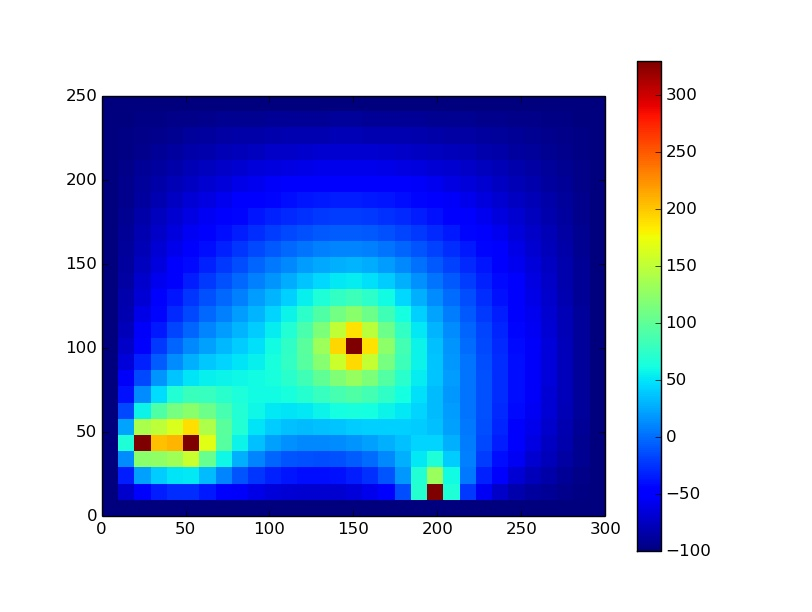
\includegraphics[scale=0.4]{E1ConH10.jpg}
	\caption{Datos usados: a=300, b=250, h=10, r=5, t=330 y k=5.}
\end{figure}


\begin{figure}[H]
\centering
  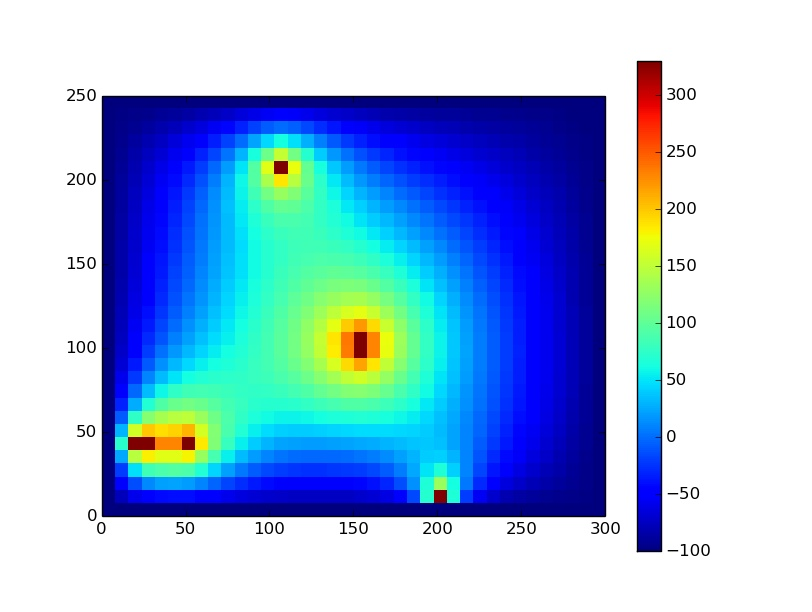
\includegraphics[scale=0.4]{E1ConH8.jpg}
	\caption{Datos usados: a=300, b=250, h= 8, r=5, t=330 y k=5.}
\end{figure}


\begin{figure}[H]
\centering
  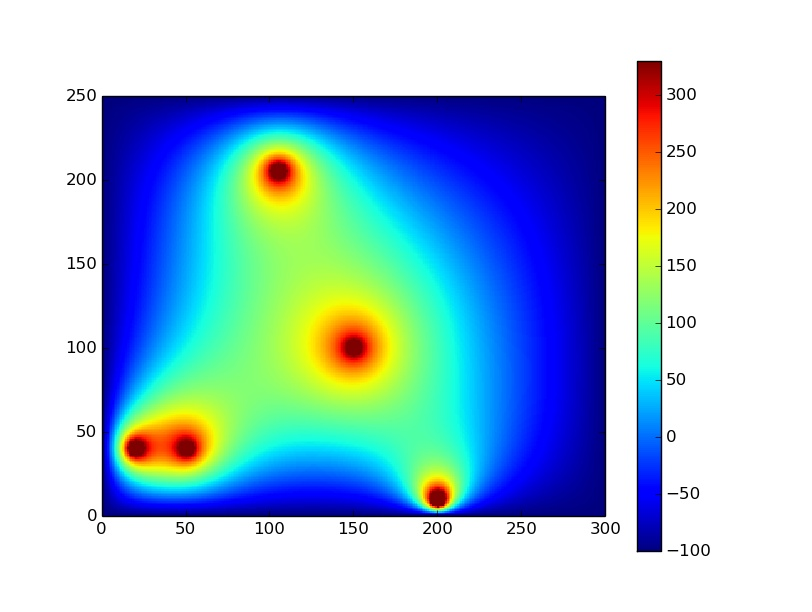
\includegraphics[scale=0.4]{E1ConH1.jpg}
 \caption{Datos usados: a=300, b=250, h=1, r=5, t=330 y k=5.}
\end{figure}

\item Segundo experimento:
\end{itemize}

\begin{figure}[H]
\centering
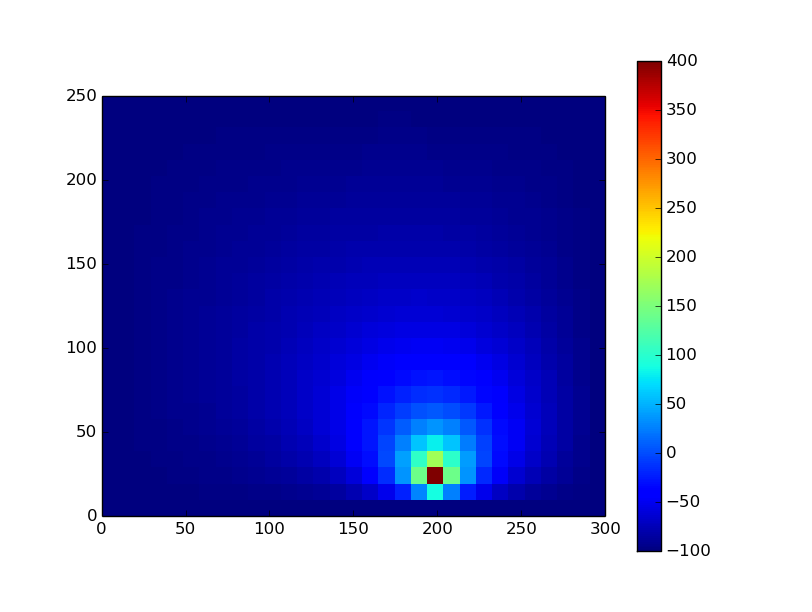
\includegraphics[scale=0.4]{E2ConH10.png}
\caption{Datos usados: a=300, b=250, h=10, r=5, t=400 y k=4.}
\end{figure}

\begin{figure}[H]
\centering
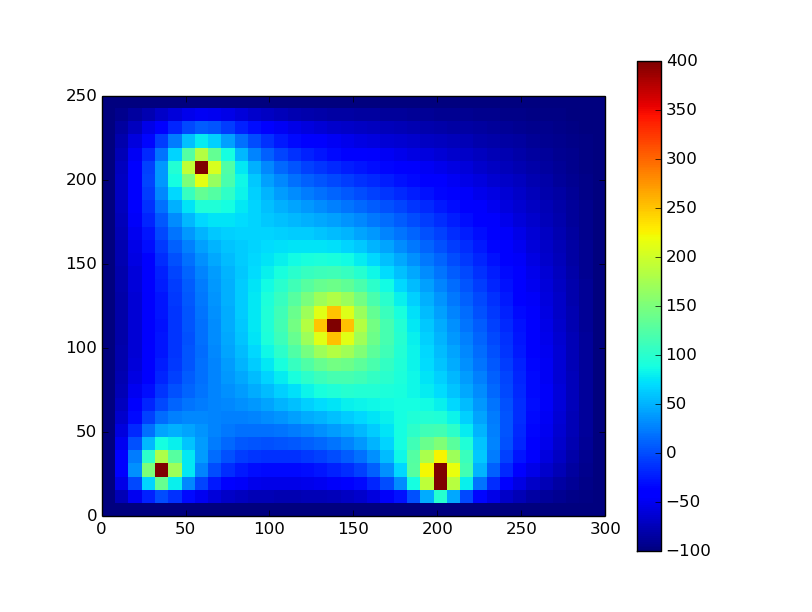
\includegraphics[scale=0.4]{E2ConH8.png}
\caption{Datos usados: a=300, b=250, h=8, r=5, t=400 y k=4.}
\end{figure}

\begin{figure}[H]
\centering
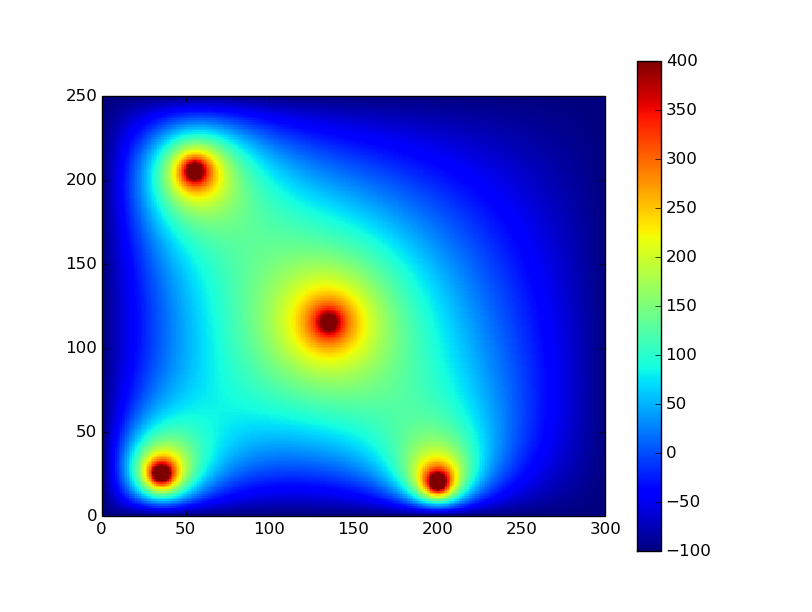
\includegraphics[scale=0.4]{E2ConH1.png}
\caption{Datos usados: a=300, b=250, h=1, r=5, t=400 y k=4.}
\end{figure}

A pesar de haber realizado varios experimentos m\'as aparte de estos 2, elegimos mostrar estos, con esos par\'ametros utilizados, debido a que la informaci\'on mostrada por los otros experimentos hechos corrobora lo que concluimos a partir de estos, sin aportar m\'as informaci\'on relevante. Es por esto que lo ocurrido en los experimentos mostrados es lo que en general suced\'io con los dem\'as. En estos, seleccionamos los param\'etros de forma tal que se puedan observar claramente el impacto que tiene realizar modificaciones en el \textit{h}, principalmente eligiendo la cantidad y posici\'on de las sanguijuelas, junto con su radio con este objetivo en mente. Aparte, elegimos los diferentes \textit{h} con el fin de que se pueda observar mejor el impacto que tiene realizar modificaciones en este, mostrando lo ocurrido con el mismo experimento con distintos valores para este param\'etro.

Al analizar los experimentos realizados pudimos ver que la granularidad afecta notablemente las temperaturas obtenidas. Una de las razones de esto es que, tal como se puede observar en el experimento 1, puede ocurrir que al ser el \textit{h} demasiado grande hay sanguijuelas que no se toman en cuenta porque no afectan a ninguno de los puntos obtenidos a partir de la discretizaci\'on (lo cual sucede en este experimento con la sanguijuela que se encuentra m\'as arriba que todas las otras). Adem\'as pudimos ver que cuanto menor es el \textit{h}, mayor es la cantidad de puntos que se toman en cuenta en la discretizaci\'on por lo tanto es m\'as cercano a lo que realmente ocurre con el parabrisas. La raz\'on de esto \'ultimo es que al realizar las diferencias finitas para obtener las ecuaciones lineales, se puede observar que cuanto menor es el \textit{h}, m\'as cerca son las aproximaciones de la derivada con este m\'etodo por lo que m\'as cercana es la temperatura obtenida. En el experimento 2 se puede observar claramente que ocurre esto, debido a que en este cuando \textit{h=10} la temperatura del punto cr\'itico es completamente err\'onea debido a que el radio afectado por cada sanguijuela es menor al \textit{h}.

Como vimos, el c\'alculo de la temperatura mejora para todos los puntos dentro de la discretizaci\'on realizada al disminuir el \textit{h}, siendo especialmente importante que lo mismo ocurra con el punto cr\'itico. La raz\'on por la que la temperatura de este punto es tan importante es que si esta es demasiado alta se romper\'a el parabrisas, por lo que es de mucha importancia que su c\'alculo sea efectuado correctamente. El motivo por el cual mejora su estimaci\'on si disminuye el \textit{h} es que, al igual que con los dem\'as puntos, esto ocasiona que se tomen una mayor cantidad de puntos en la discretizaci\'on ocasionando que m\'as cercano se encuentre el parabrisas discretizado al parabrisas real.

En conclusi\'on, pudimos observar en los experimentos realizados acerca de la granularidad utilizada que el uso de \textit{h} distintos, pueden tener un impacto notable sobre lo cercano que se encuentra el modelo que estamos representando (la discretizaci\'on realizada) de lo que realmente ocurre. Esto se debe a que cuanto menor sea el valor de este par\'ametro, mejores ser\'an las estimaciones realizadas, por lo que no solo sera m\'as cercana la temperatura calculada para cada punto discretizado con respecto a la del parabrisas real, sino que tambi\'en del punto cr\'itico.

\subsection{Tiempo de c\'omputo}

Luego de los anteriores experimentos, pasamos a centrarnos en analizar diferentes aspectos de nuestros algoritmos realizacionados con el tiempo que estos tardan en ejecutarse. Primero, al ya tener dos formas alternativas de representar las matrices con las que trabajamos pasamos a comparar estas en base al tiempo y al espacio que cada una de ellas requiere para su funcionamiento, centrandonos especialmente en ver si es que pudimos aprovechar que las matrices con las que trabajamos son matrices banda. Es decir, tratamos de ver si es que mediante nuestra representaci\'on alternativa de las matrices de este estilo pudimos ahorrar tiempo y/o espacio en nuestros algoritmos. Aparte, como ya analizamos el impacto que la granularidad tiene sobre la calidad de las temperaturas obtenidas, quisimos ver como este modifica el tiempo de ejecuci\'on utilizado. Con el objetivo de realizar apropiadamente estos experimentos, repetimos 25 veces cada uno, calculando el promedio de los tiempos en segundos obtenidos (sacando para esto 4 outliers, es decir los 2 menores valores obtenidos y los 2 mayores). La raz\'on por la que realizamos de esta forma nuestros experimentos es que puede ocurrir que alguna de las veces que los realizamos haya algo externo al programa que estamos corriendo (otro programa o un aumento o disminuci\'on de la velocidad del CPU) que ocasione que alguna de las mediciones realizadas sea muy distinta del valor real, estas las quitamos al sacar los outiliers.

\subsubsection{An\'alisis de la forma de representar la matriz}

Empezamos primero comparando las dos maneras alternativas que tenemos de representar las matrices y los algoritmos que utilizamos para trabajar con ellas. Para esto, comparamos dos distintos aspectos de estos, el tiempo y el espacio requerido para que estos funcionen. Empezamos primero analizando el tiempo, para lo cual realizamos una serie de experimentos, variando diferentes par\'ametros del programa, centrandonos principalmente en modificar la cantidad de sanguijuelas y el tamaño del parabrisas con el que trabajamos, manteniendo los demas par\'ametros constantes. La raz\'on por la que realizamos esto es que, al analizar los algoritmos utilizados pudimos ver que la temperatura no modifica en nada el tiempo de c\'omputo debido a que solo ocasiona un cambio en el valor inicial de \textit{b}. Por otro lado, el radio de las sanguijuelas no lo modificamos debido a que la cantidad de puntos del parabrisas discretizado afectados por sanguijuelas la modificamos con la cantidad de estas \'ultimas, no con su tamaño. Adem\'as, el tamaño de las matrices con las trabajamos lo modificamos realizando cambios con el \textit{a/b} y no con el \textit{h} por lo que este lo mantenemos constante. Esto se debe a que el \textit{h} modificar\'ia el tamaño al aumentar o disminuir los valores de \textit{n} y \textit{m}, lo cual explicamos con m\'as detalle al realizar los experimentos de tiempo con respecto a la granularidad. 

Teniendo en cuenta lo anterior, realizamos diferentes experimentos, variando en estos el tamaño de las matrices con las que trabajamos (cambiando el valor de \textit{a} y de \textit{b}) as\'i como tambi\'en la cantidad de sanguijuelas y el m\'etodo para representar las matrices. En estos, con el fin de que las sanguijuelas esten distribuidas uniformemente en el parabrisas, establecimos su posici\'on aleatoriamente. Al leer los algoritmos implementados para cada uno de los m\'etodos realizados para representar las matrices, nosotros preve\'iamos que al realizar estos experimentos iba a haber una gran diferencia en el tiempo que tarda en realizarse cada uno de los experimentos para cada uno de estos. La raz\'on por la que pensabamos esto es que, a pesar de que parece no haber tanta diferencia entre lo realizado en el algoritmo para resolver las matrices, en los otros dos si que hay diferencias notorias. En primer lugar, la principal diferencia en el algoritmo de creaci\'on de la matriz es que para las matrices tradicionales no aprovechamos el hecho que los vectores vienen inicializados en cero, por lo que debimos recorrer toda la matriz para incializarla, algo que no realizamos para la matriz banda. Por otro lado, debido al menor tamaño de las matrices banda, en el algoritmo de eliminaci\'on gaussiana debimos realizar menos operaciones puesto que solo operamos con los coeficientes guardados en la matriz en ambos casos (que en el caso de la matriz banda es una cantidad mucho menor). Aparte, en el caso de la matriz banda, hay veces que no realizamos ninguna operaci\'on muy costosa si no es necesario, es decir si un coeficiente ya esta en cero no realizamos ninguna operaci\'on con este, mientras que para las matrices tradicionales siempre realizamos una resta entre las filas. Adem\'as, la resta de filas es una operaci\'on mucho m\'as costosa en el caso de tratarse de una matriz tradicional debido a que las filas en estas son de largo \textit{n*m} mientras que para las matrices bandas es de \textit{2*n+1}, aparte de que al realizar la resta para estas \'ultimas solo restamos \textit{n} coeficientes (debido a que aprovechamos que gran parte de la matriz se encuentra en cero).

Por estas razones es que nosotros cre\'iamos que iba a haber una gran diferencia de tiempo al comparar el tiempo de c\'omputo requerido para ambos m\'etodos, sin importar el valor de los demas par\'ametros. Luego de realizar una serie de experimentos, algunos de los resultados obtenidos fueron los siguientes (estos no fueron los \'unicos realizados pero si los que reflejan claramente lo ocurrido en general:

\begin{figure}[H]
\centering
	\subfigure[Matriz Tradicional]{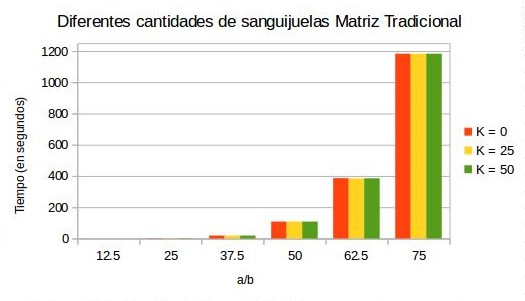
\includegraphics[scale=0.5]{CSMT.jpg}}
	\subfigure[Matriz Banda]{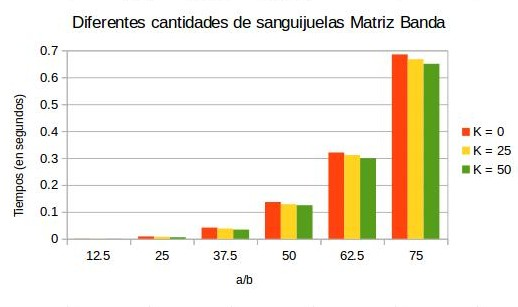
\includegraphics[scale=0.5]{CSMB.jpg}}
	\subfigure[Matriz Tradicional vs Matriz Banda]{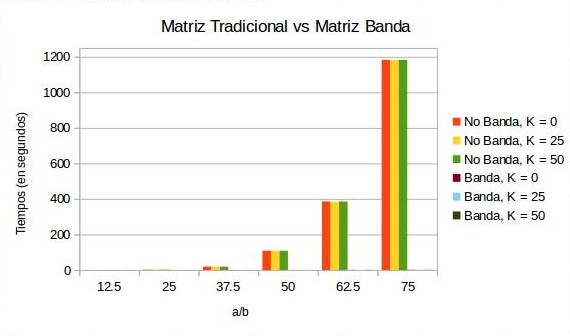
\includegraphics[scale=0.5]{MTvsMB.jpg}}
	\caption{Tiempos Matriz Tradicional vs Matriz Banda} 
\end{figure}

Tal como se puede en los gr\'aficos, nuestra hip\'otesis era correcta, debido a que se puede ver que hay una amplia diferencia en el tiempo tardado para cada los dos m\'etodos, pudiendo no verse el tiempo tardado por en el caso de la matriz banda en comparaci\'on con el uso de la matriz tradicional. Por otro lado, tambi\'en se puede observar que parece haber una relaci\'on cuadr\'atica entre el tamaño de las matrices y el tiempo que tardan los algoritmos en realizarse, debido a que este va aumentando muy r\'apidamente a medida que aumentamos el tamaño de las matrices, siendo esto m\'as notorio para la representaci\'on tradicional de las matrices. Aparte, algo muy importante que se puede observar en los gr\'aficos es que a medida que vamos aumentando la cantidad de sanguijuelas, hay una disminuci\'on en el tiempo de c\'omputo requerido para realizar las operaciones con la matriz banda (aunque esta cantidad no es tan grande), manteniendose este valor con poca variaci\'on para la matriz tradicional.

Luego de ese an\'alisis pasamos a ver que tal era el ahorro de espacio utilizando el m\'etodo de representaci\'on alternativo para las matrices en vez del tradicional. Al ver los algoritmos vimos que para la matriz tradicional, como guardamos todos los datos, esta pertenece a $\mathbb{R}^{n*m \times n*m}$ es decir que debe utilizar \textit{($n^{2}$)*($m^{2}$)} lugares para guardar la informaci\'on. A diferencia de esta, la matriz banda es de $\mathbb{R}^{n*m \times 2*n+1}$ entonces ocupa \textit{n*m*(2*n+1)} (lo que es igual a \textit{2*($n^{2}$)*m+n*m = O($n^2$*m}). Luego representando la matriz de esta forma se ahorra memoria.

En conclusi\'on pudimos ver, luego de este an\'alisis, que la representaci\'on alternativa de las matrices supera en todo aspecto a la tradicional, siendo mucho mejores sus algortimos en cuanto al tiempo y al espacio, sin importar el tamaño de matriz con el que trabajemos. Es por esto que recomendamos la utilizaci\'on de esta forma alternativa de representar la matriz antes que la tradicional. Por otro lado, tambi\'en pudimos una ver disminuci\'on en el tiempo requerido a medida que aumentabamos la cantidad de sanguijuelas en el parabrisas para las matrices banda (sin modificar ning\'un otro par\'ametro), as\'i como tambi\'en la existencia de una relaci\'on cuadr\'atica entre los tiempos requeridos por cada uno de los m\'etodos y el tamaño de las matrices.

\subsubsection{Granularidad}

Luego, continuamos analizando que ocurr\'ia al modificar la granularidad con la que trabajamos en cada una de las formas de representar la matriz. Con este fin, en nuestros experimentos dejamos fijos la cantidad, posici\'on y radio de cada una de las sanguijuelas (tomando siempre 25 sanguijuelas de radio 1 con su posici\'on elegida aleatoriamente), haciendo lo mismo con la temperatura de las sanguijuelas pero cambiando el tamaño del parabrisas con el que trabajamos como as\'i tambi\'en la granularidad. La raz\'on por la que utilizamos una cantidad de sanguijuelas constante es que, como vimos en el experimento anterior, la cantidad con la que trabajemos tiene muy poca influencia en el tiempo que tardan los algoritmos. Adem\'as elegimos su posici\'on aleatoria debido a que de esta manera las sanguijuelas estan distribuidas uniformemente en el parabrisas (lo que igual no tiene tanta importancia por lo anteriormente mencionado). Por otro lado, mantuvimos constante la temperatura que las sanguijuelas ocasionan que tenga el parabrisas debido a que esta no influye en el trabajo de nuestros algoritmos.

Teniendo en cuenta todo lo anterior, realizamos una serie de experimentos viendo en estos que ocurr\'ia al trabajar con parabrisas con distintas discretizaci\'on (es decir con un \textit{h} distinto), analizando esto para ambas formas de representar la matriz y diferentes tamaños de esta. Nuestra hip\'otesis al realizar estos experimentos era que sin importar como vayamos variando estos \'ultimos (es decir la forma de representar la matriz y su tamaño), siempre iba a ocurrir que el tiempo de c\'omputo aumente a medida que disminuyamos el \textit{h} (si es que mantenemos todos los demas par\'ametros constantes). La raz\'on por la que pensabamos esto es que el tamaño de las matrices con las que trabajamos es inversamente proporcional al \textit{h}, lo que se debe a que el tamaño de las matrices sea $\mathbb{R}^{n*m \times n*m}$ o $\mathbb{R}^{m*n \times 2*n+1}$, valiendo:

\begin{center}
$m = \dfrac{b}{h}+1$ \\
$n = \dfrac{a}{h}+1$
\end{center}

Luego, al disminuir \textit{h} aumentan \textit{n} y \textit{m} por lo que a su vez tambi\'en lo hace el tamaño de la matriz en ambos casos, lo cual ocasionar\'ia que el tiempo de c\'omputo requerido para trabajar con esta sea mayor. Es por esta raz\'on que nosotros supusimos que un \textit{h} menor iba a ocasionar que, para ambas formas de representar la matriz y para cualquier tamaño, el tiempo que los algortimos tarden en ejecutarse sea mayor. Luego para probar si nuestra hip\'otesis era correcta realizamos una serie de experimentos, siendo algunos de ellos:

\begin{figure}[H]
\centering
	\subfigure[Matriz Tradicional]{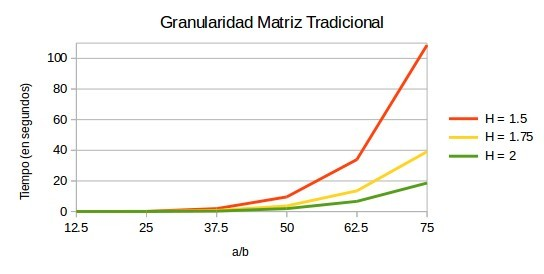
\includegraphics[scale=0.5]{GMT.jpg}}
	\subfigure[Matriz Banda]{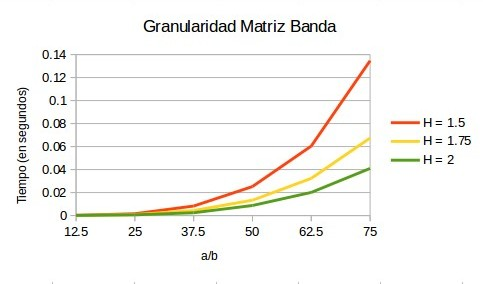
\includegraphics[scale=0.6]{GMB.jpg}}
	\caption{Granularidad} 
\end{figure}

A pesar de haber realizado otros experimentos aparte de los mostrados en el informe, en todos los realizados obtuvimos siempre los mismos resultados, por lo que se puede observar en los casos mostrados lo que en general ocurre. Entonces, la raz\'on por la que en estos elegimos \textit{h=1.5}, \textit{h=1.75} y \textit{h=2} es debido a que muestran lo que ocurren para diferentes \textit{h} y porque si variabamos demasiado su valor entonces la diferencia en tiempo se hacia tan grande que no se podia observar con claridad lo que ocurr\'ia con los tiempos (al menos en los gr\'aficos, en los valores obtenidos los resultados eran los mismos).

Al analizar lo ocurrido, pudimos ver que ocurr\'ia lo que nosotros habiamos pensado, es decir que sin importar el tamaño de la matriz con la que trabajemos ni si esta es la matriz banda o matriz tradicional, siempre aumenta el tiempo de c\'omputo a medida que disminuimos el \textit{h} (a pesar de que algunos de estos no se pueden ver con claridad en los gr\'aficos). Otra cosa importante de mencionar es que este experimento sigue confirmando m\'as lo ocurrido en el experimento de comparaci\'on de las distintas formas de representar las matrices. Esto se debe a que hay una amplia diferencia entre el tiempo que tarda en realizarse los experimentos entre ambas formas de representar la matriz, siendo siempre el tiempo superior para la representaci\'on tradicional de la matriz, ocurriendo esto a\'un cuando comparamos para diferentes \textit{h} con el mismo tamaño.

\subsection{Punto Cr\'itico y Eliminaci\'on de Sanguijuelas}
En este apartado se discutir\'a sobre el comportamiento de la estimaci\'on del punto cr\'itico y el algoritmo de eliminar sanguijuelas. Si bien ya hemos explicado como realizamos ambos m\'etodos, nos gustar\'ia discutir sobre si son eficientes o no, y cu\'ales son sus ventajas y desventajas.

Luego de los experimentos realizados, se puede ver que al tener intervalos de discretizaci\'on m\'as pequeños, la temperatura de cada punto va a ser m\'as acertada y que al estimar la temperatura del punto cr\'itico vamos a estar m\'as cerca del valor real. Por ejemplo, si es que nos encontramos en el caso en el que el punto cr\'itico cae dentro de unos de los puntos discretizados, si nuestros intervalos de discretizar son pequeños, vamos a estar muy cerca del valor real, pero si estos intervalos son muy grandes, entonces no van a estar muy bien representados los valores de las temperaturas y la del punto cr\'itico no va a ser muy parecida al valor real buscado. Algo similar sucede en el caso en el que el punto cr\'itico no cae dentro de los puntos de discretizaci\'on. Como estamos tomando el promedio, si nuestro intervalo es tan pequeño que cada valor de la temperatura de cada punto se acerca mucho al de la realidad, luego al tomar el promedio de estos puntos tambi\'en estaremos cerca de encontrar el valor de la temperatura del punto cr\'itico. En cambio, si el intervalo de discretizaci\'on es muy grande, como los puntos no est\'an reflejando muy bien la temperatura real, entonces la temperatura del punto cr\'itico tampoco va a estar muy bien reflejada. Por ende, se puede concluir que la temperatura del punto cr\'itico que estimamos depende m\'as del tamaño del intervalo de discretizaci\'on que del m\'etodo propuesto. 

Cuando nos encontramos en el algoritmo de eliminaci\'on de sanguijuelas, es un m\'etodo aproximado para realizar lo pedido y no exacto. Uno de las desventajas que tenemos, lo cual afecta en la exactitud, es que se puede dar el caso en el que, cuando el punto cr\'itico no cae sobre un punto de la discretizaci\'on, puede suceder que dado 2 puntos cercanos (cuando m era par y n era impar o viceversa, m era impar y n era par. Tambi\'en puede suceder esto cuando son 4 los puntos cercanos, solo exhibimos un ejemplo.), llam\'emoslos \textit{x} e \textit{y}, \textit{x} tenga muchas sanguijuelas que lo engloben mientras que \textit{y} solo contenga una. Dependiendo de como est\'en pasadas en el .in que tomamos como archivo de entrada estas sanguijuelas, nuestro algoritmo lo que puede llegar a hacer es primero eliminar todas las sanguijuelas que se encuentren sobre el punto \textit{x} menos una, en este caso cada punto \textit{x} y \textit{y} tienen solo una sanguijuela actualmente, y lo que sucedi\'o es que la temperatura de nuestro punto cr\'itico todav\'ia no disminuy\'o, dado que las sanguijuelas encimadas no acumulan su temperatura, y reci\'en en el pr\'oximo paso disminuir al eliminar la siguiente sanguijuela. Por esta raz\'on es que este m\'etodo no es exacto y, a veces, no muy eficiente. Una forma de corregir este problema ser\'ia primero verificando de todos los puntos cercanos al punto cr\'itico, aquel que tenga menos sanguijuelas englob\'andolo y primero eliminar todas esas; de esta forma nos aseguramos que el punto cr\'itico disminuya su temperatura lo m\'as r\'apido posible para que as\'i el parabrisas no se destruya. Tambi\'en otra forma de solucionarlo podr\'ia ser par\'andonos en cualquiera de estos puntos cercanos y eliminar todas las sanguijuelas que est\'en afect\'andolo actualmente en un paso. Otro problema que tiene nuestro algoritmo es que repetitivamente vamos buscando aquellas sanguijuelas que se encuentran dentro del radio \textit{r}, lo que implica que si nos dieron \textit{x} sanguijuelas cuya ubicac\'ion es dentro de este radio, entonces \textit{x} veces estaremos recorriendo los vectores que contienen las sanguijuelas buscando aquellas que se encuentren cercanas y siempre encontrar\'iamos las mismas. Esto se podr\'ia resolver modificando un poco nuestro algoritmo de la siguiente manera (reemplazando nom\'as lo que se encuentra dentro del \textit{while}):

\vspace{5mm}
\begin{algorithm}[H]
	\textbf{entero} cantidadSanguijuelas\;
	Buscar sanguijuelas que se encuentren a radio \textit{radio} y colocar la cantidad encontrada en el entero cantidadSanguijuelas\;
	\While{Hay sanguijuelas en el radio}{
		Eliminar una\;
		Disminuir cantidadSanguijuelas\;
		Calcular temperaturas de los puntos discretizados\;
		Calcular temperatura del punto critico\;
		\If{Temperatura \textless \ 235\hspace{-1.5mm}$\phantom{a}^{\circ}$C}{
			cantidadSanguijuelas = 0\;
		}	
	}	
	Radio = Radio + $\frac{h}{4}$\;		

\caption{Mejora del algoritmo de Eliminacion de Sanguijuelas}
\end{algorithm}	

Las ventajas de nuestro m\'etodo es que, al crearnos un radio alrededor del punto cr\'itico e ir aument\'andolo, esto nos asegura de ir agarrando primero los puntos m\'as cercanos a \'este, luego ir agarrando los siguientes m\'as cercanos y etc. De esta forma, siempre vamos a ir eliminando las sanguijuelas que m\'as directamente est\'en afectando la temperatura del punto cr\'itico, para as\'i poder eliminar todas las m\'as cercanas necesarias para que vaya disminuyendo la temperatura. Cabe aclarar que si realizacemos lo de encontrar primero los puntos con menos sanguijuelas de aquellos puntos m\'as cercanos con sanguijuelas, o eliminar de cada punto todas las sanguijuelas que lo afecten de un solo paso, luego nuestro m\'etodo ser\'ia mucho m\'as eficiente y podr\'iamos colocar esto dentro de las ventajas de nuestro m\'etodo puesto que estar\'iamos m\'as acertados con cu\'ales sanguijuelas eliminasemos. 

Si bien como explicamos anteriormente este m\'etodo puede no funcionar bien en algunos casos, si la distribuci\'on de las sanguijuelas fuese uniforme, habr\'ia menos probabilidad de caer en el caso en el que sobre uno de los puntos cercanos hubiese muchas sanguijuelas y sobre los otros pocas, y que nuestro algoritmo primero eliminase todas las sanguijuelas sobre ese punto que contiene mayor cantidad. Esto se debe a que estar\'ian mejor distribuidas alrededor de todo el parabrisas, entonces al suceder esto la probabilidad de que muchas caigan sobre un punto ser\'ia baja y tambi\'en la probabilidad de que aquellas que vinieron encimadas hayan sido dadas consecutivamente (puesto que nuestro algoritmo de eliminaci\'on va eliminando aquellas que primero encontr\'o en en el vector \textit{x} e \textit{y}). Entonces si nos encontrasemos en este caso, nuestro algoritmo de eliminaci\'on de sanguijuelas ser\'ia mucho m\'as efectivo ya que no caer\'iamos tan frecuentemente en aquellos casos en los que no funciona tan bien. 

Luego de realizar el an\'alisis anterior, vamos a hablar de los experimentos realizados sobre nuestro algoritmo de eliminar sanguijuelas para evaluar su funcionamiento. Lo que se buscaba observar era que efectivamente estuviese eliminando las sanguijuelas cercanas al punto cr\'itico y no las que no lo afectaban, y adem\'as que la temperatura final del punto cr\'itico no se encuentre en peligro. Por esto, esto es lo que esperamos ver en las im\'agenes.

Hemos realizado este experimento con varias muestras distintas, decidiendo mostrar solamente 2 de ellas ya que reflejaban bien el comportamiento esperado del algoritmo. Para estos seleccionamos 30 sanguijuelas coloc\'andolas en lugares particulares (en los bordes, cerca del punto cr\'itico y algunas m\'as concentradas en la regi\'on entre el punto cr\'itico y los bordes) para ver si eran eliminadas o no. Adem\'as, en estas dos instacias que mostraremos, hemos cambiado el valor de la temperatura que ejerce cada sanguijuela (240\hspace{-1.5mm}$\phantom{a}^{\circ}$C para el primer experimento y 500\hspace{-1.5mm}$\phantom{a}^{\circ}$C para el segundo). Tomamos un ancho y largo del parabrisas de 250 metros, con una granularidad de 1 y un radio de 5 metros sobre el cual las sanguijuelas ejercen el calor. Tambi\'en hemos calculado la temperatura del punto cr\'itico al finalizar la ejecuci\'on del algoritmo para evaluarla. Hemos obtenido los siguientes gr\'aficos:

\begin{figure}[H]
\centering
	\subfigure[Sin eliminar sanguijuelas]{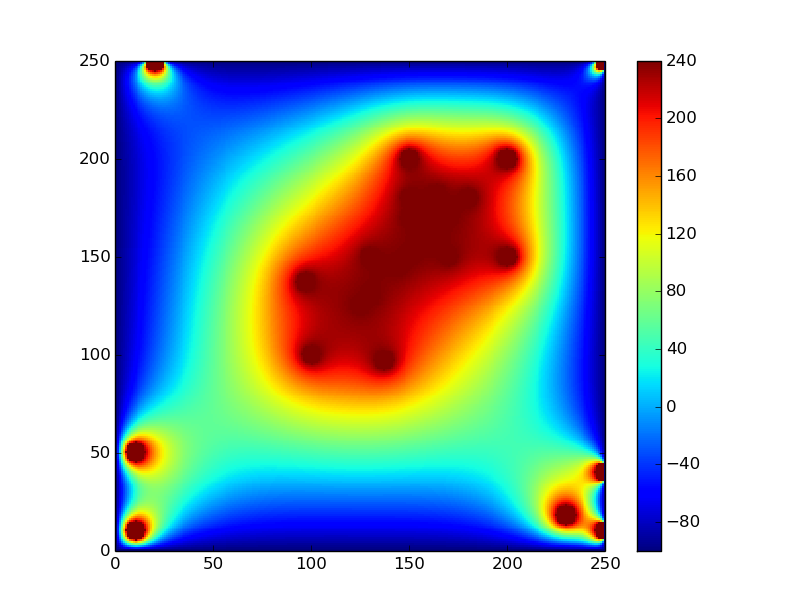
\includegraphics[scale=.35]{test11}}
	\subfigure[Eliminando sanguijuelas]{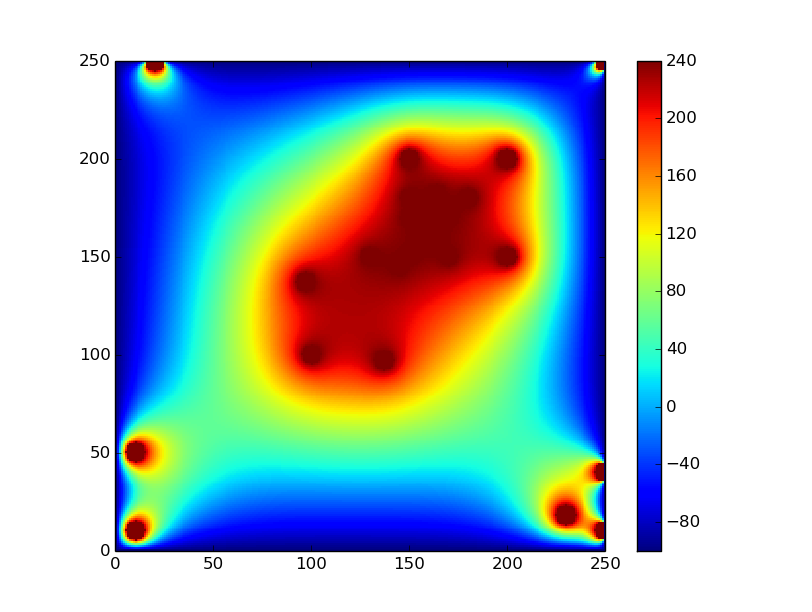
\includegraphics[scale=.35]{test12}}
	\caption{Experimento 1} 
\end{figure}

\begin{figure}[H]
\centering
	\subfigure[Sin eliminar sanguijuelas]{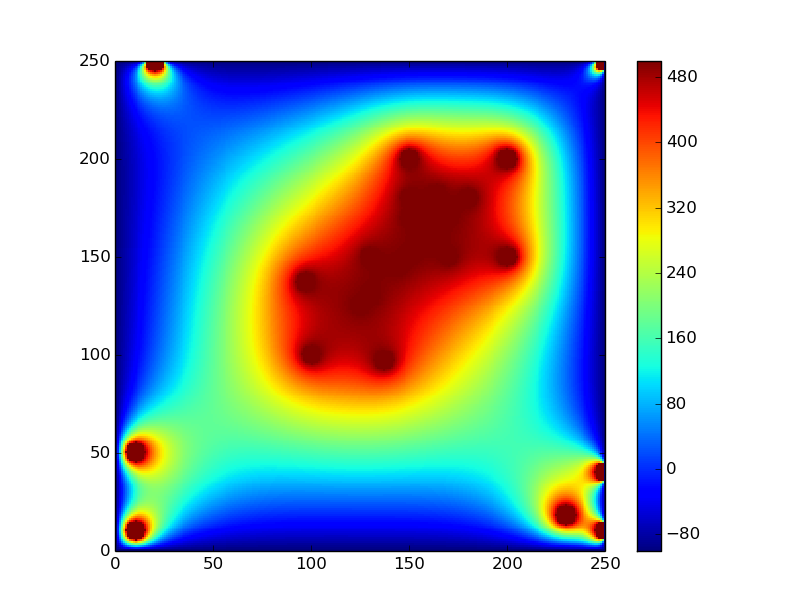
\includegraphics[scale=.35]{test31}}
	\subfigure[Eliminando sanguijuelas]{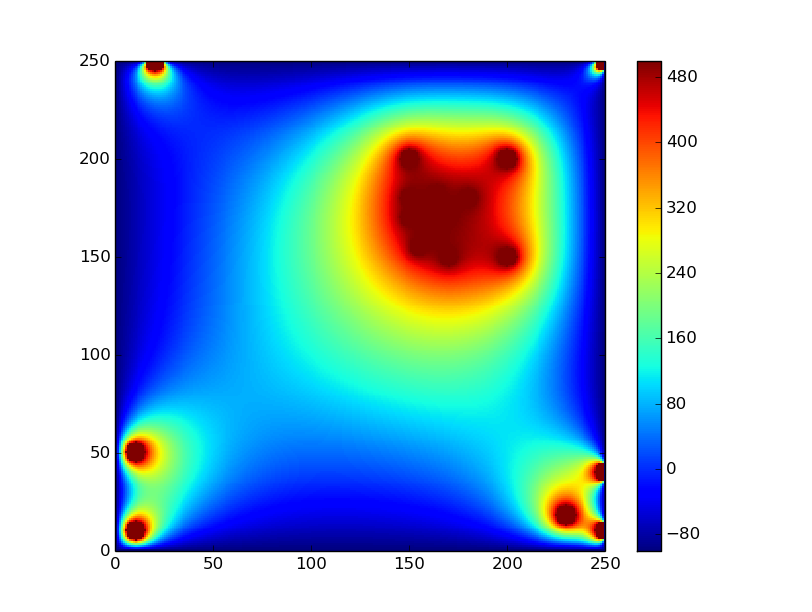
\includegraphics[scale=.35]{test32}}
	\caption{Experimento 2} 
\end{figure}



En el primero de los experimentos, en el cual las sanguijuelas ejerc\'ian una temperatura de 240\hspace{-1.5mm}$\phantom{a}^{\circ}$C, podemos observar c\'omo cambio la temperatura de la zona en la que se encontraba el punto cr\'itico (en la posici\'on $(125.5;125.5)$), el cual pas\'o de tener varias sanguijuelas cercanas que generaban una temperatura elevada all\'i a tener una zona m\'as despejada. Luego del experimento la temperatura final del punto cr\'itico fue de 226,52\hspace{-1.5mm}$\phantom{a}^{\circ}$C, lo cual nos lleva a concluir que fueron eliminadas las sanguijuelas para que la temperatura disminuyera de los 235\hspace{-1.5mm}$\phantom{a}^{\circ}$C. 

En el segundo, en el cual las sanguijuelas ejerc\'ian una temperatura de  500\hspace{-1.5mm}$\phantom{a}^{\circ}$C, se puede observar mejor que muchas m\'as sanguijuelas fueron eliminados puesto que provocaban una mayor temperatura en el punto cr\'tico. Se puede ver que este punto qued\'o totalmente despejado de sanguijuelas puesto que, al ejercer una temperatura tan alta, si hubiese alguna cercana provocar\'ia que el punto cr\'itico estuviese en problemas. Adem\'as, la temperatura final de este punto fue de 233,689\hspace{-1.5mm}$\phantom{a}^{\circ}$C, lo cual efectivamente elimin\'o las necesarias para que no este m\'as en peligro. 

De ambos experimentos pudimos sacar las mismas conclusiones, las cuales fueron que se eliminaron correctamente todas las sanguijuelas debidas para que la temperatura del punto cr\'itico bajase del valor pedido. En el segundo caso, esta eliminaci\'on fue mayor debido a que, como las sanguijuelas ejerc\'ian mayor temperatura, hab\'ian m\'as afectando al punto cr\'itico que deb\'ian ser eliminadas. Aparte, en ambos gr\'aficos se pueden observar que todas las dem\'as sanguijuelas de puntos lejanos se mantuvieron intactas, es decir que no fueron eliminadas por nuestro algoritmo, confirmando nuestras hip\'otesis iniciales. Por esto, y por los dem\'as experimentos realizados que mostraron situaciones similares, podemos confirmar que nuestro algoritmo efectivamente elimina las sanguijuelas m\'as cercanas al punto cr\'itico que provocan que su temperatura se encuentre en estado grave, es decir mayor o igual a 235\hspace{-1.5mm}$\phantom{a}^{\circ}$C, haciendo que nuestro m\'etodo funcione correctamente. 

\newpage
\section{Conclusion}

En conclusi\'on, a lo largo de este trabajo pr\'actico realizamos distintas implementaciones de las matrices banda (junto con todos los algoritmos utilizados para resolver el sistema de ecuaciones lineales al que esta asociada) con el fin de poder solucionar el problema de como calcular la temperatura de los puntos del parabrisas. Adem\'as, realizamos an\'alisis de estas (mediante una serie de experimentos), llegando a las conclusiones de que pudimos pensar una estructura alternativa para representar a la matriz banda, debido a la utilizaci\'on de esta ocasiona que haya un ahorro en el tiempo y en el espacion utilizado. Adem\'as analizamos que ocurr\'ia en ambos casos cuando se modificaba la granularidad viendo que si \textit{h} era mayor se perd\'ian datos y que los resultados obtenidos se iban haciendo m\'as lejanos de lo que realmente ocurr\'ia, perjudicando a su vez el c\'alculo de la temperatura en el punto cr\'itico, aunque esto ocasionaba que el tiempo de c\'omputo sea menor. Con respecto al punto cr\'itico, podemos concluir que la estimaci\'on de su temperatura depende m\'as del tamaño de los intervalos de discretizaci\'on que del m\'etodo propuesto. Puede suceder que, al tener un intervalo muy grande, esta estimaci\'on no sea buena. Pero en el mejor caso nos estaremos acercando al valor real buscado. Si bien a veces este punto no cae dentro de los puntos discretizados, creemos que nuestra forma de obtenerlo es bastante eficaz. Con respecto al m\'etodo de eliminaci\'on de sanguijuelas, ya hemos discutido sus ventajas y desventajas. Luego de la realizaci\'on de varios experimentos podemos concluir que la eficacia de nuestro m\'etodo est\'a relacionada a la distribuci\'on de las sanguijuelas en el parabrisas. Puede suceder que nuestro m\'etodo no sea muy eficiente como tambi\'en serlo bastante. Tambi\'en podr\'iamos lograr que este sea eficiente en la mayor\'ia de los casos aplicando varias modificaciones en nuestro algoritmo, las cuales ya fueron nombradas anteriormente.

\newpage

\section{Modificaciones}
Al realizar este trabajo pr\'actico, realizamos algunas modificaciones a algunos de los algortimos comunmente usados por distintos motivos, por ejemplo, para que sean m\'as f\'aciles de implementar. Las modificaciones que realizamos fueron:
\begin{itemize}
\item Realizamos una modificaci\'on al algoritmo de eliminaci\'on gaussiana al adaptar este para su uso en matrices banda, esta la realizamos con el objetivo de que sea m\'as f\'acil de implementar. Lo que cambiamos es que en vez de realizar implementar este como normalmente es, es decir, en cada paso del algortimo poner en cero todos los valores debajo de la diagonal para cada columna (tal como lo hicimos para la eliminaci\'on gaussiana para cuando guardamos la matriz de la forma tradicional), nos centramos en cada paso en que esto suceda para cada fila. Entonces, en cada paso de este algoritmo, lo que hacemos es usar las filas que se encuentran m\'as arriba de con la que estamos trabajando ahora para que en la fila en la que nos encontremos queden en ceros todos coeficientes que se encuentran anteriores a la diagonal. Utilizando la forma alternativa para representar las matrices, esto significa que luego de cada paso poseeremos una fila m\'as de la matriz banda con los primeros \textit{n} coeficientes en cero.
\end{itemize}

\end{document}